\documentclass[12pt,a4paper,oneside]{report}
\usepackage[utf8]{inputenc}
\usepackage[T1]{fontenc}
\usepackage{textcomp}
\usepackage[margin=2.5cm]{geometry}
\usepackage{setspace}
\onehalfspacing
\setlength{\emergencystretch}{3em}
\usepackage{graphicx}
\usepackage{amsmath}
\usepackage{amssymb}
\usepackage{booktabs}
\usepackage{longtable}
\usepackage{tabularx}
\usepackage{array}
\usepackage{enumitem}
\usepackage{hyperref}
\hypersetup{colorlinks=true, linkcolor=blue, citecolor=blue, urlcolor=blue}
\usepackage{csquotes}
\usepackage[backend=biber, style=authoryear, natbib=true]{biblatex}
\addbibresource{references.bib}
\usepackage{cleveref}
\usepackage{tikz}
\usetikzlibrary{shapes,arrows,positioning,calc,decorations.pathreplacing,fit,matrix,backgrounds,mindmap}
\usepackage{pgfplots}
\pgfplotsset{compat=1.18}
\usepackage{algorithm2e}
\usepackage{appendix}
\usepackage{fancyhdr}
\usepackage{listings}
\usepackage{xcolor}
\lstset{
  basicstyle=\ttfamily\small,
  breaklines=true,
  columns=fullflexible,
  frame=single,
  keepspaces=true,
  showstringspaces=false
}

\pagestyle{fancy}
\fancyhf{}
\chead{\textit{Paila Nepal: AI-Driven Offline-First Tourism Mobile Application}}
\rfoot{\thepage}
\setlength{\headheight}{15pt}

\title{\textbf{Paila Nepal:\\An Offline-First Rural Tourism Mobile Application\\for Gandaki Province, Nepal}\\[1.2cm]\large Individual Honours Project Report}
\author{Abhishek Paudel \\ Student ID: 23140737 \\[0.8cm] BSc (Hons) Computer and Data Science \\ Birmingham City University \\[0.8cm] Module: CMP6200 \\ Supervisor: Sumanta Silwal \\ Word Count: 8,000}
\date{May 2026}

\begin{document}

\pagenumbering{roman}
\hypersetup{pageanchor=false}
\maketitle
\hypersetup{pageanchor=true}

\newpage
\chapter*{Abstract}

Paila Nepal is an offline-first rural tourism mobile application designed to provide destination discovery, map access, route guidance, and personalized recommendations for travelers exploring Gandaki Province, Nepal, particularly in regions with limited or unstable internet connectivity. The application addresses a critical gap in existing tourism platforms: most popular map and travel applications rely on continuous internet access and are optimised for well-known commercial destinations, leaving rural tourism locations with inadequate digital representation.

This project implements a Flutter-based Android application supported by a FastAPI backend, bundling 300 curated Gandaki Province destinations, 771 accommodation records, local photographs, descriptions, structured attributes, and precomputed semantic embeddings. The final recommendation architecture combines SBERT semantic retrieval, collaborative and popularity signals, contextual reranking, machine-learning rescoring, cold-start handling, diversity control, and explanation generation. The mobile application preserves recommendation capability offline using local embeddings and contextual scoring. Local persistence uses SQLite for saved destinations and reviews, Hive for recommendation caches, preferences, and queued interactions, and SharedPreferences for lightweight settings. A bundled MBTiles package provides offline map display. The chatbot combines local language processing, hybrid intent classification, retrieval-augmented response generation, emergency detection, dialogue memory, translation support, and optional online language-model enhancement.

Evaluation used five tourism recommendation scenarios and the ranking metrics Precision@10, Recall@10, normalised Discounted Cumulative Gain at 10, and Mean Reciprocal Rank. The hybrid recommender achieved average Precision@10 of 0.6800, Recall@10 of 0.4408, nDCG@10 of 0.7543, and MRR of 1.0000. Current automated verification also shows that Flutter static analysis passes and nine backend tests pass. The full Flutter suite exposed one remaining widget-test lifecycle issue, while a focused performance test showed that warm offline translation exceeded its 500 ms target on the test machine. These findings support the viability of the architecture while identifying concrete limitations for further improvement.

Paila Nepal demonstrates how offline-first mobile architecture, combined with curated rural tourism content, can improve information accessibility and travel safety for rural tourism in Nepal. The project achieves a balance between comprehensive feature richness and practical offline reliability, contributing to both academic understanding of offline-first design patterns and practical tools for rural tourism promotion.

\textbf{Keywords:} rural tourism, Flutter, offline-first architecture, Gandaki Province, MBTiles, OSRM routing, SQLite, recommendation systems, chatbot, OpenStreetMap, mobile application design.

\newpage
\chapter*{Acknowledgements}

I would like to express my sincere gratitude to Sumanta Silwal, my supervisor at Birmingham City University, for his guidance, constructive feedback, and encouragement throughout this project. His insights on system design, offline-first architecture, and mobile application development have been invaluable.

I am grateful to the Faculty of Computing, Engineering and the Built Environment at Birmingham City University for providing a rigorous academic environment and access to resources necessary for this work. The course CMP6200: Individual Honours Project has allowed me to integrate knowledge from multiple domains---software engineering, data structures, mobile development, and tourism informatics---into one cohesive system.

I acknowledge the open-source community for the technologies that made this project possible: Flutter, FastAPI, OpenStreetMap, OSRM, SQLite, and MBTiles. These tools embody principles of openness and accessibility that align with the goals of rural tourism development.

Finally, I dedicate this work to the communities and destinations of Gandaki Province, Nepal, whose tourism potential I hope this application helps to advance.

\newpage
\tableofcontents
\newpage
\listoffigures
\newpage
\listoftables

\chapter*{Abbreviations}
\begin{table}[h]
\centering
\begin{tabular}{ll}
\toprule
\textbf{Abbreviation} & \textbf{Meaning} \\
\midrule
API & Application Programming Interface \\
APK & Android Package \\
CRUD & Create, Read, Update, Delete \\
GPS & Global Positioning System \\
HTTP & Hypertext Transfer Protocol \\
IDE & Integrated Development Environment \\
JSON & JavaScript Object Notation \\
MBTiles & Map Box Tiles \\
FAISS & Facebook AI Similarity Search \\
Hive & Local key-value database used by the Flutter application \\
MRR & Mean Reciprocal Rank \\
nDCG & Normalised Discounted Cumulative Gain \\
NLP & Natural Language Processing \\
OSRM & Open Source Routing Machine \\
RAG & Retrieval-Augmented Generation \\
SBERT & Sentence-BERT \\
SQLite & Structured Query Language Lite \\
UI & User Interface \\
UX & User Experience \\
WebP & Efficient modern image format \\
XYZ & Tile coordinate system (tile.openstreetmap.org/{z}/{x}/{y}) \\
TMS & Tile Map Service \\
\bottomrule
\end{tabular}
\end{table}

\newpage
\clearpage
\pagenumbering{arabic}
\chapter{Introduction}
\label{ch:introduction}

\section{Background and Motivation}
\label{sec:background}

Tourism is an important economic and cultural sector in Nepal, generating employment, foreign exchange, and opportunities for regional development \parencite{NepalTourism2023}. Gandaki Province contains Pokhara, a major tourism gateway, alongside rural villages, mountains, lakes, trekking routes, cultural settlements, and pilgrimage sites. Yet digital coverage is concentrated on Pokhara and famous routes, while many rural destinations remain poorly represented.

This information gap is intensified by unreliable connectivity. Travelers moving through rural Gandaki frequently encounter weak mobile data, high bandwidth costs, power disruption, and inconsistent internet access at accommodation. Most mainstream tourism platforms assume a continuous connection: they download content on demand, stream images, and request live routes. When the network fails, maps, descriptions, accommodation details, recommendations, and assistance can disappear together.

Paila Nepal is motivated by the principle that rural travel support should remain useful without continuous internet access. It therefore treats locally stored information and computation as the operational foundation, using the network to enhance results when available. This is the central idea of offline-first design.

\section{Problem Statement}
\label{sec:problem}

Rural travelers in Gandaki Province face three connected problems. First, geographic context and navigation can disappear when map tiles and live route requests fail. Second, many destinations lack structured information about activities, accessibility, budgets, seasons, culture, family suitability, adventure level, and nearby accommodation. Third, general-purpose maps, booking platforms, and review aggregators do not prioritise Gandaki's villages, homestays, viewpoints, or low-connectivity travel conditions. These weaknesses create uncertainty for travelers and reduce the visibility and potential economic benefit of rural destinations.

The core problem addressed by this project can be stated as follows:

\begin{center}
\textit{How can a mobile application provide offline-capable destination discovery, map access, route guidance, personalized recommendations, and tourism assistance for Gandaki Province rural tourism, particularly in contexts where internet connectivity is unreliable or unavailable?}
\end{center}

Addressing the problem requires more than cached maps. It requires bundled destination data and media, local map tiles, route caching and fallback computation, local tourism intelligence, persistent storage, meaningful destination attributes, and optional online enhancement.

\section{Project Aim and Objectives}
\label{sec:objectives}

The primary aim of this project is to design and implement a Flutter-based Android mobile application that provides offline-first rural tourism support for Gandaki Province, demonstrating how offline-first architecture can enhance digital accessibility in low-connectivity tourism contexts.

The specific objectives are:

\begin{enumerate}
\item To build a fully offline-capable Flutter mobile application for Android that launches, displays destination data, supports map exploration, provides route guidance, and answers tourism queries without requiring internet connectivity.

\item To curate and integrate a structured dataset of 300 rural tourism destinations in Gandaki Province, including geographic coordinates, categories, activities, seasonality, budget levels, accessibility ratings, family-friendliness indicators, adventure levels, cultural attributes, nature attributes, descriptions, tags, and image references.

\item To bundle local destination photographs using optimised WebP compression (approximately 300 images), allowing destination cards, list views, and detail screens to display rich visual content offline.

\item To integrate a local MBTiles raster map package focused on Gandaki Province (zoom levels 7--12), enabling users to browse Pokhara and surrounding rural areas without downloading tiles at runtime.

\item To implement a three-tier routing architecture: (1) SQLite route cache for previously-requested routes, (2) online OSRM routing when internet is available, and (3) offline Haversine straight-line route computation as a fallback.

\item To implement an offline-capable chatbot using local language processing, hybrid intent classification, knowledge retrieval, dialogue memory, emergency detection, structured response generation, and optional online LLM enhancement.

\item To provide explainable personalized destination recommendations using semantic embeddings, contextual matching, cold-start handling, diversity filtering, interaction-derived collaborative signals, and machine-learning reranking.

\item To support persistent user data including saved destinations, reviews, recommendation caches, queued interactions, and preferences through SQLite, Hive, and SharedPreferences.

\item To integrate a FastAPI backend for online enhancements including AI chatbot responses, advanced recommendations, user authentication, and analytics, while preserving core local functionality.

\item To evaluate the application through offline functionality testing, performance analysis, user experience assessment, and critical evaluation of design decisions and limitations.
\end{enumerate}

\section{Scope and Limitations}
\label{sec:scope}

The project focuses on Gandaki Province, particularly destinations accessible from Pokhara. Its 300 curated destination records provide meaningful coverage while remaining practical for offline distribution. The bundled raster map covers zoom levels 7--12; extending this to street-level detail across every village would make the application substantially larger.

Routing uses OSRM for road-aware instructions when online, cached routes when available, and a Haversine approximation when disconnected. The fallback is useful for direction and distance estimation, but it is not offline turn-by-turn navigation. The local chatbot does not run an LLM on-device; instead, it combines multilingual text processing, hybrid intent classification, retrieval, dialogue state, safety rules, and templates, with optional cloud-model enhancement.

The deployment target is Android. iOS testing and distribution are outside the present scope. Other limitations include best-available photographs that may be representative rather than exact, no real-time traffic or weather, incomplete community-contribution workflows, and no bundled road graph for fully offline navigation.

\section{Report Structure}
\label{sec:report_structure}

The remaining chapters review relevant literature, present the architecture and implementation, evaluate the completed system, discuss technical challenges, and conclude with contributions, limitations, and future work.
\chapter{Literature Review}
\label{ch:literature}

\section{Rural Tourism in Nepal and Gandaki Province}
\label{sec:rural_tourism}

Rural tourism links Nepal's landscapes and cultural heritage with community-based economic development. Unlike tourism concentrated in cities or famous routes, it can distribute spending to homestays, local guides, small guesthouses, craft producers, and agricultural communities. Gandaki Province is especially important because Pokhara provides a gateway to villages such as Ghandruk, Ghorepani, Bandipur, and Sikles, as well as trekking, lake, adventure, pilgrimage, and cultural experiences.

Tourism can support livelihoods, infrastructure, conservation, and cultural preservation, but it can also create environmental pressure, dependency, and cultural commodification. Accessible and accurate information is therefore important: travelers need to understand routes, accommodation, seasons, activities, costs, culture, and safety before choosing lesser-known places. Many rural Gandaki destinations remain poorly described online, and their information often becomes inaccessible when connectivity fails.

Paila Nepal treats rural destination information as core local content. Structured attributes, photographs, maps, and supporting knowledge remain available offline and can also support recommendation and conversational assistance.

\section{Offline-First Mobile Application Architecture}
\label{sec:offline_first}

Offline-first architecture treats local data and computation as the operational foundation rather than treating disconnection as an exceptional error. The network becomes a channel for synchronisation, remote computation, fresh data, and improved results. Common patterns include reading local data first, applying local updates immediately, queueing remote operations, resolving conflicts after reconnection, communicating synchronisation state, and degrading unavailable services to useful local alternatives. SQLite suits durable relational records because it is embedded and serverless \parencite{SQLite2026}, while Flutter provides one mobile codebase with access to storage and mapping packages \parencite{Flutter2026}.

Paila Nepal applies these patterns by bundling 300 destination records and local WebP images, storing raster maps in MBTiles, caching routes in SQLite, computing a Haversine fallback, running local tourism intelligence, and persisting saved places, reviews, preferences, and queued interactions. This combination allows the user interface and core local workflows to remain available while remote services are unreachable.

MBTiles is central to the mapping strategy because it stores tiled map data in one SQLite-based container rather than thousands of separate files. This simplifies distribution, validation, and version management. The map derives from OpenStreetMap data \parencite{OpenStreetMap2026}, while OSRM supplies road-network routes when online \parencite{OSRM2026}. The project's \texttt{pokhara.mbtiles} file is approximately 7.79 MB and covers the focused area at several zoom levels.

\section{Recommendation Systems in Tourism}
\label{sec:recommendation_systems}

Recommendation systems help users navigate large collections by suggesting items predicted to be relevant or interesting. In tourism contexts, recommender systems can suggest destinations, attractions, accommodations, activities, routes, or trip plans based on user preferences and contextual factors.

Tourism recommendation is more complex than recommending generic products because travel decisions involve multiple interconnected dimensions: geographic distance, seasonality, budget, activity preferences, cultural interests, family composition, physical accessibility, adventure tolerance, weather conditions, and personal mood. A destination that is ideal for a solo trekker may be unsuitable for a family with young children. A destination attractive in autumn may be dangerous during monsoon. Budget-conscious tourists need different recommendations than luxury travelers.

The first prototype of Paila Nepal used content-based filtering, in which destination attributes were compared directly with user preferences. This was appropriate during early development because content-based methods remain usable during cold start, when a newly installed application has no interaction history. However, a purely content-based design risks overspecialisation and cannot learn effectively from user behaviour. Recommender-system literature therefore identifies hybridisation as a practical way to combine the strengths of different signals while reducing their individual weaknesses \parencite{Adomavicius2005,Burke2002}.

The destination dataset supports content-based filtering through category, activities, best season, budget, accessibility, adventure level, family suitability, cultural richness, nature score, tags, and descriptive text.

A recommendation algorithm computes a match score between user preferences and each destination's attributes. For example, if a user indicates preferences for ``trekking in autumn with moderate budget and family-friendly options,'' the system can score destinations by measuring alignment with these criteria. High-scoring destinations are recommended first. Diversity constraints can ensure that recommendations include varied destination types rather than clustering on a single category.

The final Paila Nepal recommender is hybrid. On the backend, a natural-language preference query is encoded using Sentence-BERT, which is designed to produce semantically meaningful sentence embeddings suitable for similarity comparison \parencite{Reimers2019}. Candidate destinations are retrieved through a normalised embedding index using FAISS when available and a NumPy dot-product fallback otherwise. Retrieval scores are then combined with structured activity and category signals. A collaborative component uses stored interactions when a user has sufficient history; popularity provides a limited cold-start prior. A contextual reranker evaluates season, budget, activity, vibe, accessibility, family suitability, adventure preference, and accommodation fit. Finally, a trained LightGBM LambdaRank model can rescore the candidates, while a fixed-weight fallback preserves operation when no trained model is available. The application also generates human-readable reasons so that users can inspect why a destination was recommended.

The mobile offline recommender uses precomputed destination embeddings and contextual attributes stored in application assets. Its first stage combines semantic embedding similarity with contextual fit, after which constraint penalties, local affinity signals, and diversity limits are applied. This differs from the earlier TF--IDF and simple cosine-similarity prototypes discussed in the interim submission: those prototypes established the feasibility of local ranking, while the final implementation uses richer semantic vectors and a broader set of contextual signals. TF--IDF nevertheless remains an important baseline because it represents text through weighted term frequency rather than semantic meaning \parencite{Salton1988}.

Tourism recommendation literature emphasises the importance of context and personalisation. \cite{Tkalcic2019} discuss context-aware recommendation systems, emphasising how travel recommendations must account for season, weather, company (solo, family, group), and activity preferences. \cite{Ye2010} examine location-based recommendation systems, noting that geographic proximity and user activity patterns significantly influence tourism recommendations.

\section{Natural Language Processing and Chatbots for Tourism}
\label{sec:nlp_chatbots}

Chatbots in tourism applications serve various functions: answering frequently-asked questions, providing contextual information, facilitating bookings, offering safety guidance, and providing translation services. Advanced chatbots using large language models (LLMs) can engage in fluent natural conversation and provide nuanced responses to varied questions.

However, cloud-based LLMs create a dependency on internet connectivity and API availability. In a system designed for offline-first rural tourism, relying entirely on cloud AI would reproduce the same connectivity vulnerability that the project is addressing. A practical alternative is to implement local natural language processing using bounded resources.

Bounded local chatbots generally combine a domain knowledge base, intent classification, entity extraction, response templates, and fallback handling. Their scope is narrower than a cloud LLM, but their behaviour is predictable, testable, private, and independent of API availability.

The earliest chatbot prototype used a local knowledge base, keyword matching, and structured templates. The final application expands this into a modular offline intelligence pipeline. English, Devanagari Nepali, and romanised Nepali text is normalised, tokenised, stemmed, enriched with synonyms, and analysed for named entities. Hybrid intent classification and semantic/BM25-style retrieval produce grounded answers, while dialogue state, slot filling, clarification questions, and memory support multi-turn interaction. It answers questions about seasons, budgets, family suitability, transport, and activities. A safety layer runs before normal response generation, ensuring that messages such as ``I'm lost'' or ``I'm injured'' receive deterministic emergency guidance.

When backend connectivity and API keys are configured, the chatbot can request online language-model enhancement. The enhancement is applied to the locally generated answer rather than replacing the complete local pipeline. However, the offline chatbot remains the reliable base layer. This design follows the offline-first principle: cloud enhancement is available when possible, but is not required for core operation. The implementation also distinguishes backend reachability from provider availability so that the interface does not incorrectly imply that online AI is active when only fallback logic is available.

\section{Related Work in Tourism Applications}
\label{sec:related_work}

Several existing applications and systems are relevant to Paila Nepal:

Google Maps provides extensive navigation and points of interest, but its richer services remain connectivity-dependent and are not focused on rural destination discovery. TripAdvisor supplies reviews and commercial tourism content but is primarily online. OSMAnd provides strong offline maps and navigation without curated Gandaki tourism assistance. Komoot and AllTrails support outdoor route discovery, yet focus mainly on hiking and community trails. Local tourism-board guides may provide regional information, but their data coverage and offline functionality vary.

\cref{tbl:related_work} compares these systems against Paila Nepal along several dimensions.

\begin{table}[h]
\centering
\small
\begin{tabular}{lcccccc}
\toprule
\textbf{System} & \textbf{Offline} & \textbf{Gandaki} & \textbf{Chatbot} & \textbf{Recommen.} & \textbf{Routing} & \textbf{Saved} \\
& \textbf{Maps} & \textbf{Focus} & & & & \\
\midrule
Google Maps & Partial & No & No & No & Yes & Yes \\
TripAdvisor & No & No & No & Yes & No & Yes \\
OSMAnd & Yes & No & No & No & Yes & No \\
Komoot & Yes & No & No & No & Yes & Yes \\
AllTrails & Partial & No & No & No & No & Yes \\
Paila Nepal & Yes & Yes & Yes & Yes & Yes & Yes \\
\bottomrule
\end{tabular}
\caption{Comparison of tourism applications and Paila Nepal. ``Offline Maps'' indicates whether offline map display is supported. ``Gandaki Focus'' indicates rural Gandaki destination specialisation. ``Chatbot'' indicates conversational tourism assistance. ``Recommen.'' indicates recommendation system. ``Routing'' indicates route guidance. ``Saved'' indicates saved place functionality.}
\label{tbl:related_work}
\end{table}

The distinctive contribution of Paila Nepal is the integration of offline-first architecture, rural Gandaki tourism content specialisation, and comprehensive offline functionality (maps, routing fallback, chatbot, recommendations). This combination addresses the specific needs of rural tourism in low-connectivity environments, a gap not fully addressed by existing applications.
\chapter{System Design and Architecture}
\label{ch:design}

\section{System Architecture Overview}
\label{sec:arch_overview}

Paila Nepal follows a layered architecture separating presentation, domain, data, and service layers. This separation of concerns improves testability, maintainability, and enables offline/online behavior to be managed cleanly. \cref{fig:layered_arch} illustrates the layered architecture.

\begin{figure}[h]
\centering
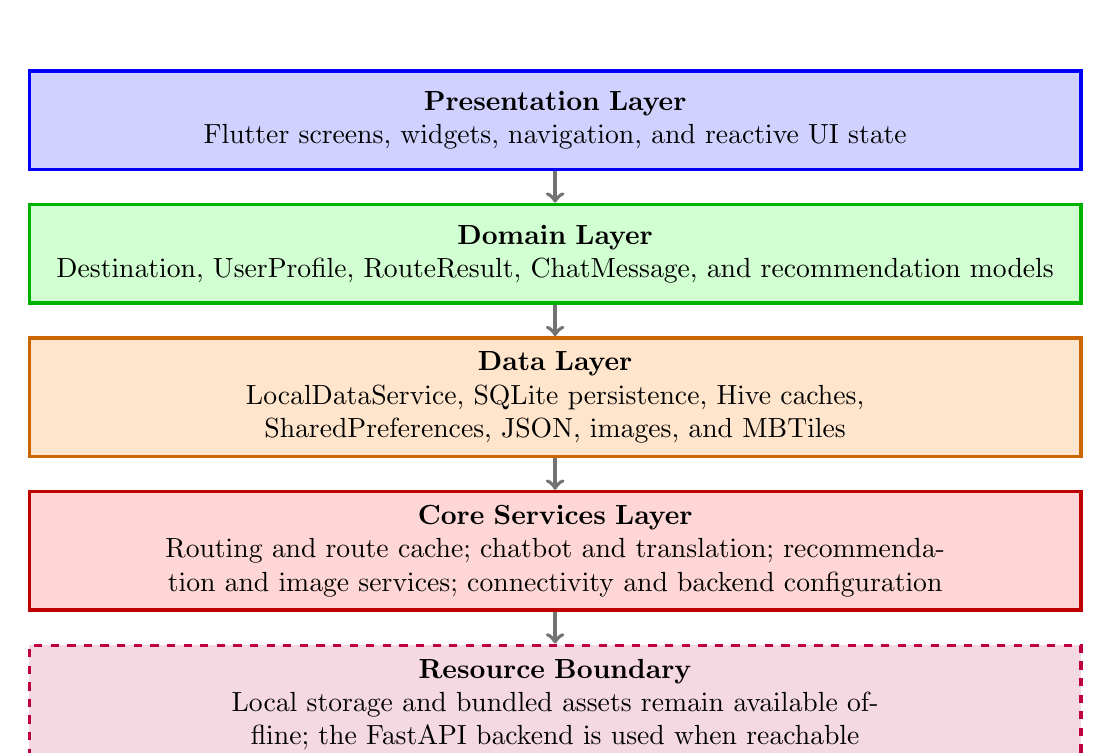
\begin{tikzpicture}[
  node distance=4mm,
  layer/.style={draw, line width=1.3pt, text width=13cm, minimum height=1.25cm, align=center, inner sep=5pt},
  flow/.style={->, line width=1.4pt, color=black!55}
]
  \node[layer, fill=blue!18, draw=blue] (presentation)
    {\textbf{Presentation Layer}\\Flutter screens, widgets, navigation, and reactive UI state};
  \node[layer, fill=green!18, draw=green!70!black, below=of presentation] (domain)
    {\textbf{Domain Layer}\\Destination, UserProfile, RouteResult, ChatMessage, and recommendation models};
  \node[layer, fill=orange!20, draw=orange!80!black, below=of domain] (data)
    {\textbf{Data Layer}\\LocalDataService, SQLite persistence, Hive caches, SharedPreferences, JSON, images, and MBTiles};
  \node[layer, fill=red!16, draw=red!75!black, below=of data] (services)
    {\textbf{Core Services Layer}\\Routing and route cache; chatbot and translation; recommendation and image services; connectivity and backend configuration};
  \node[layer, fill=purple!15, draw=purple, dashed, below=of services] (resources)
    {\textbf{Resource Boundary}\\Local storage and bundled assets remain available offline; the FastAPI backend is used when reachable};

  \draw[flow] (presentation) -- (domain);
  \draw[flow] (domain) -- (data);
  \draw[flow] (data) -- (services);
  \draw[flow] (services) -- (resources);
\end{tikzpicture}
\caption{Layered system architecture. The application separates presentation logic, domain models, data persistence, and core services. Services access both local resources (storage, assets) and optional external backend services. This separation enables offline-first operation.}
\label{fig:layered_arch}
\end{figure}

The \textbf{Presentation Layer} consists of Flutter widgets, screens, UI components, dialogs, bottom sheets, and navigation logic. Examples include the home screen, destination list, destination detail view, map screen, chatbot interface, recommendations screen, and settings screens. The presentation layer receives input from users and displays output by rendering widgets. It communicates with services and providers to retrieve data and trigger actions.

The \textbf{Domain Layer} contains entities and models representing core application concepts. Examples include:

\begin{itemize}
\item \texttt{Destination} model with attributes: id, name, description, latitude, longitude, category, activities, best\_season, budget\_level, accessibility, adventure\_level, family\_friendly, cultural\_richness, nature\_score, tags, image\_url.
\item \texttt{UserProfile} model with preferences: interests, budget, adventure\_level, family\_status.
\item \texttt{RouteResult} model with: origin, destination, distance, duration, polyline, steps, is\_fallback.
\item \texttt{ChatMessage} model with: content, sender (user/chatbot), timestamp, intent.
\item \texttt{RecommendationResult} model with: recommended\_destinations, scores, reasoning.
\end{itemize}

Domain models define the structure of data independently of UI or persistence concerns. This ensures that data can move between services, screens, and storage mechanisms in a type-safe manner.

The \textbf{Data Layer} manages all local and remote data access. It includes:

\begin{itemize}
\item \texttt{LocalDataService}: Loads destinations and accommodations, manages SQLite records for saved destinations, reviews, events, and profiles, and coordinates Hive-backed recommendation data.
\item Asset loading: JSON files containing destination data, chatbot knowledge bases, phrasebooks, embeddings.
\item \texttt{HiveStorageService}: Stores recommendation caches, user preferences, local interactions, and interactions queued for backend synchronisation.
\item \texttt{SharedPreferences}: Lightweight key-value storage for settings and web fallbacks.
\item Image services: Access to destination images stored as WebP assets and cached network images.
\item MBTiles provider: Access to offline map tiles via \texttt{flutter\_map\_mbtiles}.
\end{itemize}

The \textbf{Services Layer} contains cross-cutting logic that coordinates lower layers:

\begin{itemize}
\item \texttt{RoutingService}: Coordinates route retrieval from cache, online OSRM, or fallback Haversine computation.
\item \texttt{IntelligenceOrchestrator}: Coordinates multilingual normalisation, intent classification, entity recognition, hybrid retrieval, dialogue state, safety checks, translation, and optional online enhancement.
\item \texttt{OfflineTileProvider}: Validates and loads MBTiles file for map display.
\item \texttt{ImageService}: Coordinates image loading from assets, cache, or backend.
\item \texttt{OfflineProvider} and \texttt{BackendConfig}: Distinguish general connectivity, backend reachability, and the availability of online enhancement.
\item \texttt{RecommenderService} and \texttt{RecommendationApiService}: Provide offline semantic/contextual ranking and access to the backend hybrid recommender.
\item \texttt{InteractionSyncService}: Queues local interactions and synchronises them in batches when the backend becomes available.
\item \texttt{BackendConfigService}: Manages backend API configuration, authentication, and availability.
\end{itemize}

This layered architecture supports offline-first operation because most presentation features depend on local services and persistent data first. The backend provides enhancement and synchronisation but is not a dependency for core functionality.

\section{Feature-Based Code Organisation}
\label{sec:feature_org}

In addition to the layered architecture, Paila Nepal uses feature-based code organisation, grouping related screens, models, services, and widgets into feature modules. This improves modularity and allows individual features to be developed and tested semi-independently.

Key feature modules include:

\begin{itemize}
\item \textbf{features/destinations:} Destination browsing, search, filtering, detail view, gallery view, and saved destination management.
\item \textbf{features/map:} Interactive map with route display, marker handling, map tile switching, offline map status, and navigation controls.
\item \textbf{features/chatbot and features/intelligence:} Chatbot UI, offline NLP, hybrid intent classification, RAG-style knowledge retrieval, safety handling, dialogue state, translation, and optional online enhancement.
\item \textbf{features/recommendations:} Personalised recommendation display, semantic/contextual offline ranking, backend hybrid ranking, preference management, score explanations, and recommendation caching.
\item \textbf{core/navigation and features/map:} Route request, route display, navigation UI, route caching, OSRM access, and offline route fallback indication.
\item \textbf{features/auth:} User authentication UI, login/signup screens, session management, and backend integration.
\item \textbf{features/account:} User profile, preferences, saved destinations, trip history, and settings.
\item \textbf{features/home:} Home screen, discovery feed, quick access widgets, and onboarding.
\item \textbf{features/shell:} Bottom navigation, tab layout, and overall app structure.
\end{itemize}

\begin{figure}[h]
\centering
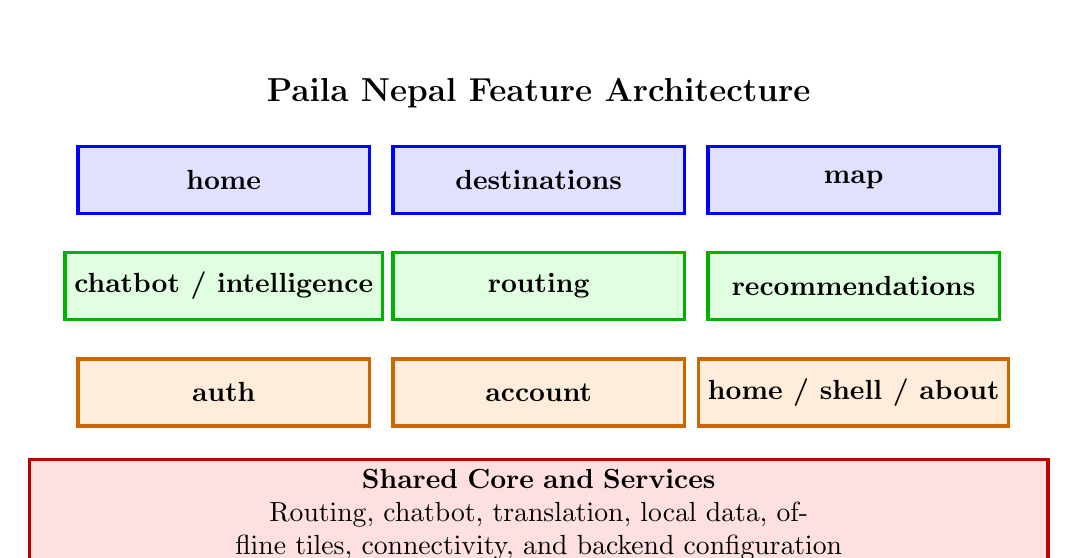
\begin{tikzpicture}[
  module/.style={draw, line width=1.2pt, minimum width=3.7cm, minimum height=0.85cm, align=center, font=\bfseries},
  shared/.style={draw=red!75!black, fill=red!12, line width=1.3pt, text width=12.7cm, minimum height=1.15cm, align=center}
]
  \node[font=\large\bfseries] at (0,1.1) {Paila Nepal Feature Architecture};

  \node[module, fill=blue!12, draw=blue] at (-4,0) {home};
  \node[module, fill=blue!12, draw=blue] at (0,0) {destinations};
  \node[module, fill=blue!12, draw=blue] at (4,0) {map};

  \node[module, fill=green!12, draw=green!70!black] at (-4,-1.35) {chatbot / intelligence};
  \node[module, fill=green!12, draw=green!70!black] at (0,-1.35) {routing};
  \node[module, fill=green!12, draw=green!70!black] at (4,-1.35) {recommendations};

  \node[module, fill=orange!14, draw=orange!80!black] at (-4,-2.7) {auth};
  \node[module, fill=orange!14, draw=orange!80!black] at (0,-2.7) {account};
  \node[module, fill=orange!14, draw=orange!80!black] at (4,-2.7) {home / shell / about};

  \node[shared] at (0,-4.25)
    {\textbf{Shared Core and Services}\\Routing, chatbot, translation, local data, offline tiles, connectivity, and backend configuration};
\end{tikzpicture}
\caption{Feature-based code organisation. Each feature module contains related screens, models, and widgets. The core/services layer provides shared functionality to all features.}
\label{fig:feature_org}
\end{figure}

\section{Offline-First Routing Architecture}
\label{sec:offline_routing}

The routing architecture is central to offline-first operation. It implements a three-tier strategy that ensures route guidance is always available, even when the online routing service is unreachable.

\textbf{Tier 1: SQLite Route Cache.} The application maintains a `RouteCache` SQLite table storing previously-computed routes. The cache key deterministically encodes the origin coordinates, destination coordinates, and travel mode. When a user requests a route, the system first checks the cache. If a valid cached entry exists (with a timestamp less than 30 days old), the cached route is returned immediately. This eliminates the need for a network request and provides instant route results.

\textbf{Tier 2: Online OSRM Routing.} If no valid cached route exists, the application attempts to retrieve an online route from the OSRM (Open Source Routing Machine) public demo server. The request includes:

\begin{itemize}
\item Origin and destination coordinates.
\item \texttt{geometries=geojson} for polygon response format.
\item \texttt{steps=true} for turn-by-turn instructions.
\item Travel mode (driving, walking, cycling).
\item HTTP timeout of 12 seconds.
\end{itemize}

If the OSRM request succeeds, the response is parsed to extract the route geometry (polyline), total distance, total duration, and step-by-step instructions. The route is then stored in the SQLite cache and returned to the user. The cache entry will provide instant results for subsequent requests to the same origin-destination pair, even if the device goes offline.

\textbf{Tier 3: Haversine Straight-Line Fallback.} If OSRM is unreachable (due to network failure, server timeout, or parsing error), the application falls back to an approximate offline route. It uses the Haversine formula to compute the great-circle distance between origin and destination. The displayed route polyline contains two points: origin and destination. Duration is estimated using travel-mode speed assumptions:

\begin{itemize}
\item Driving: 60 km/h.
\item Walking: 5 km/h.
\item Cycling: 15 km/h.
\end{itemize}

The estimated duration is computed as: $\text{duration} = \frac{\text{haversine\_distance}}{speed}$.

The route result is marked with `isFallback = true`, allowing the UI to display a warning message such as: ``This is an approximate route. Turn-by-turn navigation requires internet connectivity.'' This manages user expectations clearly.

\begin{figure}[h]
\centering
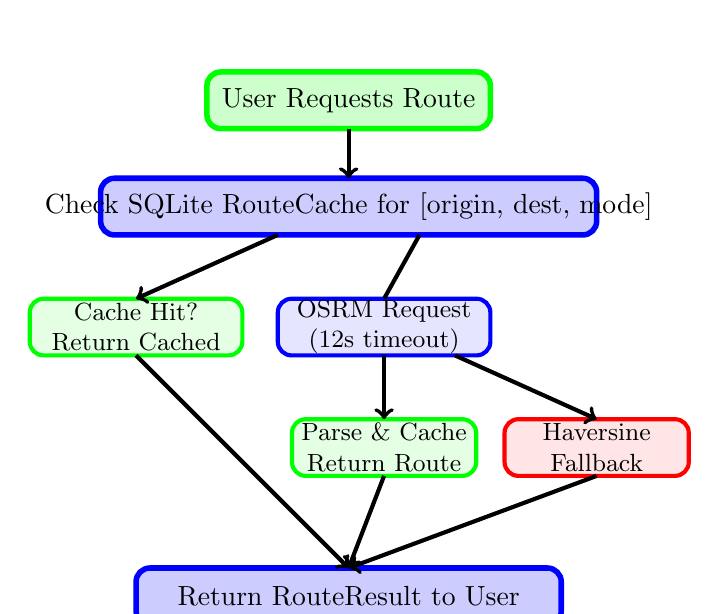
\begin{tikzpicture}[scale=0.9]
  % Start
  \draw[fill=green!20, draw=green, line width=2pt, rounded corners=5pt] (3, 10) rectangle (7, 10.8);
  \node at (5, 10.4) {User Requests Route};
  
  % Check cache
  \draw[fill=blue!20, draw=blue, line width=2pt, rounded corners=5pt] (1.5, 8.5) rectangle (8.5, 9.3);
  \node at (5, 8.9) {Check SQLite RouteCache for [origin, dest, mode]};
  
  % Cache hit
  \draw[fill=green!10, draw=green, line width=1.5pt, rounded corners=5pt] (0.5, 6.8) rectangle (3.5, 7.6);
  \node[align=center, font=\small] at (2, 7.2) {Cache Hit? \\ Return Cached};
  
  % Try OSRM
  \draw[fill=blue!10, draw=blue, line width=1.5pt, rounded corners=5pt] (4, 6.8) rectangle (7, 7.6);
  \node[align=center, font=\small] at (5.5, 7.2) {OSRM Request \\ (12s timeout)};
  
  % OSRM success
  \draw[fill=green!10, draw=green, line width=1.5pt, rounded corners=5pt] (4.2, 5.1) rectangle (6.8, 5.9);
  \node[align=center, font=\small] at (5.5, 5.5) {Parse \& Cache \\ Return Route};
  
  % OSRM fail
  \draw[fill=red!10, draw=red, line width=1.5pt, rounded corners=5pt] (7.2, 5.1) rectangle (9.8, 5.9);
  \node[align=center, font=\small] at (8.5, 5.5) {Haversine \\ Fallback};
  
  % All paths return
  \draw[fill=blue!20, draw=blue, line width=2pt, rounded corners=5pt] (2, 3) rectangle (8, 3.8);
  \node at (5, 3.4) {Return RouteResult to User};
  
  % Arrows
  \draw[->, line width=1.5pt] (5, 10) -- (5, 9.3);
  \draw[->, line width=1.5pt] (4, 8.5) -- (2, 7.6);
  \draw[-, line width=1.5pt] (6, 8.5) -- (5.5, 7.6);
  \draw[->, line width=1.5pt] (5.5, 6.8) -- (5.5, 5.9);
  \draw[->, line width=1.5pt] (6.5, 6.8) -- (8.5, 5.9);
  \draw[->, line width=1.5pt] (2, 6.8) -- (5, 3.8);
  \draw[->, line width=1.5pt] (5.5, 5.1) -- (5, 3.8);
  \draw[->, line width=1.5pt] (8.5, 5.1) -- (5, 3.8);
  
\end{tikzpicture}
\caption{Three-tier routing architecture. The system checks the SQLite route cache first, then attempts online OSRM routing if needed. If OSRM fails, a Haversine straight-line fallback is computed. All paths guarantee a route result to the user.}
\label{fig:routing_arch}
\end{figure}

This architecture ensures that users always receive route guidance, even in severely constrained connectivity situations. Cached routes provide instant results for frequently-requested routes. OSRM provides high-quality road-network routes when connectivity allows. The Haversine fallback ensures the app never fails with an error, but instead provides approximate guidance with transparent warnings.

\section{Data Architecture and Storage}
\label{sec:data_arch}

Paila Nepal uses multiple storage layers to support offline operation:

\subsection{Local Asset Data}

\texttt{assets/data/destinations.json} contains 300 curated destination records. Each destination includes:

\begin{lstlisting}
{
  "id": "destination_001",
  "name": "Ghandruk",
  "description": "A scenic Gurung village in the Annapurna foothills...",
  "latitude": 28.3956,
  "longitude": 83.8622,
  "category": "village",
  "activities": ["trekking", "village_tour", "culture"],
  "best_season": ["autumn", "spring"],
  "budget_level": "budget",
  "accessibility": "moderate",
  "adventure_level": 2,
  "family_friendly": true,
  "cultural_richness": 8,
  "nature_score": 7,
  "tags": ["gandaki", "annapurna", "gurung"],
  "image_url": "ghandruk.webp"
}
\end{lstlisting}

This JSON is loaded into memory on app startup and remains accessible offline. The data structure supports efficient searching, filtering, and recommendation scoring.

\subsection{Destination Images}

\texttt{assets/destination\_images/} contains 300 WebP format images (approximately 8.74 MB total). WebP provides better compression than JPEG or PNG, reducing the bundle size while maintaining visual quality suitable for mobile displays.

\subsection{SQLite and Hive Persistence}

The application uses two SQLite databases together with several Hive boxes. This separation reflects the different access patterns of each data type: relational records and indexed queries remain in SQLite, while typed caches and synchronisation queues use Hive.

\textbf{Main App Database} (\texttt{paila.db}):

\begin{table}[h]
\centering
\small
\resizebox{\textwidth}{!}{%
\begin{tabular}{p{4.0cm}p{4.0cm}p{6.0cm}}
\toprule
\textbf{Table} & \textbf{Columns} & \textbf{Purpose} \\
\midrule
\texttt{saved\_destinations} & id, payload, saved\_at & User-saved destinations \\
\texttt{app\_events} & id, event\_type, payload, created\_at & Local application event log \\
\texttt{destination\_reviews} & destination\_id, rating, review\_text, created\_at & Local destination ratings and reviews \\
\texttt{user\_profiles/interactions} & profile and interaction fields & Personalisation history and migration support \\
\bottomrule
\end{tabular}
}
\end{table}

\textbf{Route Cache Database} (\texttt{route\_cache.db}):

\begin{table}[h]
\centering
\small
\begin{tabular}{lll}
\toprule
\textbf{Table} & \textbf{Columns} & \textbf{Purpose} \\
\midrule
\texttt{cached\_routes} & key, data, cached\_at & Route caching (30-day TTL) \\
\bottomrule
\end{tabular}
\end{table}

\textbf{Hive Boxes:}

\begin{itemize}
\item \texttt{recommendation\_cache\_v1}: cached recommendation payloads and timestamps.
\item \texttt{user\_preferences\_v1}: the current structured recommendation preferences.
\item \texttt{user\_interactions\_v1}: local interaction history used for personalisation.
\item \texttt{pending\_backend\_interactions\_v1}: queued events waiting for batch synchronisation.
\end{itemize}

\subsection{SharedPreferences}

Lightweight key-value storage for:

\begin{itemize}
\item Selected map style.
\item Lightweight settings and web-platform fallbacks.
\item Last app version opened.
\item Offline map validation status.
\item User authentication token (if available).
\end{itemize}

\subsection{Backend API Data}

When connectivity is available, the FastAPI backend can provide:

\begin{itemize}
\item Enhanced chatbot responses via LLM integration.
\item Hybrid recommendations using SBERT retrieval, collaborative and popularity signals, contextual reranking, and optional ML rescoring.
\item User authentication and account synchronisation.
\item Interaction batch synchronisation, analytics, recommendation-quality monitoring, and model training/evaluation endpoints.
\item Image lookup and CDN delivery.
\item Trip planning suggestions.
\end{itemize}

The backend is optional for core local workflows. It enhances the experience with road-aware routing, online AI, account services, synchronisation, analytics, and the most advanced recommendation pipeline when connectivity is available.

\section{State Management with Riverpod}
\label{sec:state_mgmt}

Paila Nepal uses Flutter Riverpod for reactive state management and dependency injection. Riverpod provides a provider-based architecture in which widgets observe state changes without tight coupling to service implementations.

Example providers:

\begin{lstlisting}
// Async data provider
final destinationsProvider = FutureProvider<List<Destination>>((ref) async {
  final service = ref.watch(localDataServiceProvider);
  return service.loadDestinations();
});

// Filtered destinations based on criteria
final filteredDestinationsProvider = 
  FutureProvider.family<List<Destination>, FilterCriteria>((ref, criteria) async {
  final destinations = await ref.watch(destinationsProvider.future);
  return destinations.where((d) => d.matchesCriteria(criteria)).toList();
});

// Recommendations
final recommendationsProvider = 
  FutureProvider<List<Destination>>((ref) async {
  final prefs = ref.watch(userPreferencesProvider);
  final engine = ref.watch(recommendationEngineProvider);
  return engine.generateRecommendations(prefs);
});

// Async route computation
final routeProvider = FutureProvider.family<RouteResult, RouteRequest>((ref, request) async {
  final routing = ref.watch(routingServiceProvider);
  return routing.getRoute(request);
});
\end{lstlisting}

Local widget state (StatefulWidget) is used for transient UI state such as animation controllers, selected filters, text input, and map controller interactions. This mixed approach balances reactivity with simplicity.
\chapter{Implementation}
\label{ch:implementation}

\section{Technology Stack}
\label{sec:tech_stack}

\cref{tbl:tech_stack} summarises the primary technologies used in Paila Nepal.

\begin{table}[h]
\centering
\small
\begin{tabular}{lll}
\toprule
\textbf{Component} & \textbf{Technology} & \textbf{Version/Details} \\
\midrule
Framework & Flutter & SDK >= 3.0.0 \\
Language & Dart & 3.x \\
State Management & flutter\_riverpod & 3.3.1 \\
Maps & flutter\_map & 8.2.2 \\
Offline Tiles & flutter\_map\_mbtiles & 1.0.4 \\
Database & sqflite & 2.3.3+1 \\
Typed Local Cache & Hive / hive\_flutter & 2.2.3 / 1.1.0 \\
Connectivity & connectivity\_plus & 7.1.1 \\
Location Services & geolocator & 14.0.1 \\
HTTP Networking & http & 1.2.0 \\
Image Caching & cached\_network\_image & 3.4.1 \\
UI Fonts & google\_fonts & 6.2.1 \\
Analytics & PostHog + Sentry & posthog\_flutter 5.24.2, sentry\_flutter 9.0.0 \\
Speech & flutter\_tts + speech\_to\_text & 3.8.5 / 7.0.0 \\
Backend & FastAPI & Python 3.9+ \\
Backend Database & PostgreSQL & with SQLite fallback \\
Semantic Retrieval & Sentence-BERT + FAISS & NumPy fallback when FAISS is unavailable \\
Learning-to-Rank & LightGBM LambdaRank & Fixed weighted fallback before training \\
Backend Cache & Redis & In-memory fallback for local operation \\
\bottomrule
\end{tabular}
\caption{Primary technology stack for Paila Nepal. The application uses Flutter/Dart for mobile development, SQLite and Hive for local persistence, and FastAPI for backend services.}
\label{tbl:tech_stack}
\end{table}

\textbf{Flutter} was selected as the primary framework because it enables rapid development of polished mobile UIs, provides consistent rendering across devices, supports hot reload for development iteration, and offers plugin support for databases, location, connectivity, and maps \parencite{Flutter2026}.

\textbf{Dart} provides null-safety, async/await syntax, and strong type checking, making it well-suited for building reliable mobile applications.

\textbf{Riverpod} provides reactive state management, enabling UI to react to data changes without tightly coupling presentation logic to service implementations.

\textbf{flutter\_map} provides open-source map rendering using OpenStreetMap data, without depending on proprietary Google Maps SDK or requiring API keys.

\textbf{flutter\_map\_mbtiles} enables offline map display by reading raster tiles from local MBTiles files.

\textbf{sqflite} provides SQLite support for relational local records, while \textbf{Hive} provides typed boxes for recommendation caches, preferences, local interactions, and queued synchronisation events.

\textbf{connectivity\_plus} detects network availability, allowing the app to determine whether it should use online or offline-only paths.

\textbf{FastAPI} on the backend provides a typed Python framework for API endpoints, automatic OpenAPI documentation, and straightforward integration with the mobile client \parencite{FastAPI2026}.

\section{Offline Map Implementation}
\label{sec:map_impl}

The offline map implementation uses a local MBTiles file (\texttt{pokhara.mbtiles}, approximately 7.79 MB) containing raster PNG tiles for the focused project area. The MBTiles format is a SQLite database containing map tiles, metadata, and other data.

\subsection{Map Tile Generation}

Map tiles were generated by downloading raster PNG tiles from the OpenStreetMap tile server for the Gandaki bounding box (approximately 83.4°E to 85.2°E, 27.8°N to 29.2°N). Tiles at zoom levels 7--12 were selected to provide regional overview to destination-level detail. The tiles were aggregated into a single MBTiles SQLite database.

The MBTiles file structure includes:

\begin{itemize}
\item \textbf{Metadata table:} Key-value pairs storing map name, type, version, attribution, and bounds.
\item \textbf{Tiles table:} Records containing zoom level (z), tile column (x), tile row (y), and tile data (PNG bytes).
\end{itemize}

\subsection{Map Validation and Loading}

Before using the MBTiles file, the app validates it:

\begin{lstlisting}
Future<bool> validateMBTiles(String filePath) async {
  try {
    final file = File(filePath);
    if (!file.existsSync()) return false;
    
    final stat = file.statSync();
    if (stat.sizeSync() < 1000000) return false; // < 1MB is suspicious
    
    // Check SQLite magic header
    final bytes = file.readAsBytesSync().take(16).toList();
    final signature = String.fromCharCodes(bytes.take(13));
    return signature.startsWith('SQLite format');
  } catch (e) {
    return false;
  }
}
\end{lstlisting}

If validation succeeds, the app loads tiles using the \texttt{flutter\_map\_mbtiles} provider. If validation fails or the file is missing, the app falls back to online tile providers (OpenStreetMap, CartoDB).

\subsection{Map Controls and Styling}

The map UI includes:

\begin{itemize}
\item Zoom controls (plus/minus buttons).
\item Current location button (centers map on user's GPS position).
\item Map style selector (enabling users to switch between Voyager, Positron, Dark Matter, or offline styles).
\item Scale indicator.
\item Offline/online status indicator showing whether local MBTiles is currently being used.
\item Destination markers for browsable destinations.
\item Route polyline display overlaid on the map.
\end{itemize}

\section{Routing Service Implementation}
\label{sec:routing_impl}

The \texttt{RoutingService} orchestrates the three-tier routing strategy:

\begin{lstlisting}
class RoutingService {
  final RouteCache routeCache;
  final http.Client httpClient;
  
  Future<RouteResult> getRoute(RouteRequest request) async {
    // Tier 1: Check cache
    final cacheKey = _generateCacheKey(request);
    final cached = await routeCache.get(cacheKey);
    if (cached != null && !cached.isExpired) {
      return cached;
    }
    
    // Tier 2: Try OSRM online
    try {
      final result = await _fetchOSRMRoute(request)
          .timeout(Duration(seconds: 12));
      await routeCache.save(cacheKey, result);
      return result;
    } catch (e) {
      // Tier 3: Fallback to Haversine
      return _computeHaversineRoute(request);
    }
  }
  
  Future<RouteResult> _fetchOSRMRoute(RouteRequest request) async {
    final url = Uri.parse(
      'https://router.project-osrm.org/route/v1/driving/'
      '${request.origin.lng},${request.origin.lat};'
      '${request.destination.lng},${request.destination.lat}'
      '?geometries=geojson&steps=true&overview=full'
    );
    
    final response = await httpClient.get(url);
    if (response.statusCode == 200) {
      final json = jsonDecode(response.body);
      final route = json['routes'][0];
      
      return RouteResult(
        origin: request.origin,
        destination: request.destination,
        distance: (route['distance'] / 1000).toDouble(), // meters to km
        duration: (route['duration'] / 60).toDouble(), // seconds to minutes
        polyline: route['geometry']['coordinates'],
        steps: route['legs'][0]['steps'].map((s) => _parseStep(s)).toList(),
        isFallback: false,
      );
    }
    throw Exception('OSRM request failed');
  }
  
  RouteResult _computeHaversineRoute(RouteRequest request) {
    final distance = _haversineDistance(
      request.origin.lat, request.origin.lng,
      request.destination.lat, request.destination.lng,
    );
    
    final speedKmH = _getTravelModeSpeed(request.travelMode);
    final duration = distance / speedKmH * 60; // km / (km/h) * 60 = minutes
    
    return RouteResult(
      origin: request.origin,
      destination: request.destination,
      distance: distance,
      duration: duration,
      polyline: [
        [request.origin.lng, request.origin.lat],
        [request.destination.lng, request.destination.lat],
      ],
      steps: [],
      isFallback: true,
    );
  }
}
\end{lstlisting}

\section{Chatbot Implementation}
\label{sec:chatbot_impl}

The initial chatbot prototype used a knowledge base and simple intent patterns stored in JSON assets. The following simplified example illustrates the early design rather than the complete final implementation:

\begin{lstlisting}
{
  "intents": [
    {
      "intent": "ask_best_season",
      "patterns": [
        "what is the best time to visit",
        "when should i go",
        "best season for"
      ],
      "response_template": "The best time to visit {destination} is {season}."
    },
    {
      "intent": "ask_budget",
      "patterns": [
        "how much budget",
        "cost for",
        "price of visiting"
      ],
      "response_template": "{destination} is suitable for {budget_level} travelers."
    },
    {
      "intent": "emergency",
      "patterns": [
        "injured", "lost", "emergency", "help", "police", "ambulance"
      ],
      "response_template": "Emergency assistance may be required. Show verified Nepal emergency contacts and the user's available location."
    }
  ],
  "destinations_knowledge": [
    {
      "name": "Ghandruk",
      "facts": [
        "A scenic Gurung village in the Annapurna region",
        "Known for hospitality and homestays",
        "Traditional stone houses and terraced fields",
        "Popular for trekking and cultural tourism"
      ]
    }
  ]
}
\end{lstlisting}

The early prototype processed user input using deterministic emergency checks, intent matching, entity extraction, and template generation:

\begin{lstlisting}
class ChatbotService {
  final ChatbotKnowledge knowledge;
  
  Future<String> processUserInput(String userInput) async {
    // Emergency detection
    if (_isEmergency(userInput)) {
      return _generateEmergencyResponse();
    }
    
    // Intent classification
    final intent = _classifyIntent(userInput);
    
    // Entity extraction
    final entities = _extractEntities(userInput, intent);
    
    // Response generation
    final response = _generateResponse(intent, entities);
    
    return response;
  }
  
  String _classifyIntent(String input) {
    final lowerInput = input.toLowerCase();
    for (final intent in knowledge.intents) {
      for (final pattern in intent.patterns) {
        if (lowerInput.contains(pattern)) {
          return intent.intent;
        }
      }
    }
    return 'unknown';
  }
  
  Map<String, String> _extractEntities(String input, String intent) {
    final entities = <String, String>{};
    
    // Extract destination name
    for (final dest in knowledge.destinations) {
      if (input.contains(dest.name)) {
        entities['destination'] = dest.name;
      }
    }
    
    return entities;
  }
}
\end{lstlisting}

In the final system, \texttt{IntelligenceOrchestrator} initialises the complete offline intelligence stack. It loads the tourism knowledge repository, destination and accommodation gazetteers, intent examples, semantic embeddings, BM25 index, translation resources, and emergency contacts. Each user message passes through multilingual normalisation, tokenisation, stemming, stop-word removal, named-entity recognition, synonym expansion, hybrid intent classification, dialogue-state tracking, retrieval reranking, and response generation. The safety layer is checked before ordinary tourism logic, and every response path records the completed dialogue turn so that conversation memory remains consistent.

When the backend is available, the chatbot can request online enhancement through the actual \texttt{/chat} endpoint. The local answer and local state remain available if that request fails:

\begin{lstlisting}
Future<String> enhanceWithLLM(String userInput, String offlineResponse) async {
  try {
    final response = await http.post(
      Uri.parse('${backendUrl}/chat'),
      body: jsonEncode({
        'question': userInput,
        'language': 'en',
        'top_k': 5,
        'history': recentHistory,
      }),
      headers: {'Content-Type': 'application/json'},
    ).timeout(Duration(seconds: 5));
    
    if (response.statusCode == 200) {
      final data = jsonDecode(response.body);
      return data['answer'] ?? data['reply'];
    }
  } catch (e) {
    // Timeout or network error; use offline response
  }
  
  return offlineResponse;
}
\end{lstlisting}

\section{Recommendation Engine}
\label{sec:recommendation_impl}

The first mobile recommendation prototype scored destinations through direct attribute matching and diversity rules. The simplified listing below represents that development stage and explains the foundation described in the interim submission:

\begin{lstlisting}
class RecommendationEngine {
  final List<Destination> allDestinations;
  
  List<Destination> generateRecommendations(UserPreferences prefs) {
    // Score each destination
    final scored = allDestinations.map((dest) {
      double score = 0.0;
      
      // Category matching
      if (prefs.preferredCategories.contains(dest.category)) {
        score += 10;
      }
      
      // Activity matching
      final matchingActivities = dest.activities
          .where((a) => prefs.preferredActivities.contains(a))
          .length;
      score += matchingActivities * 2;
      
      // Budget alignment
      if (dest.budgetLevel == prefs.budgetLevel) {
        score += 5;
      }
      
      // Season appropriateness
      final currentMonth = DateTime.now().month;
      final currentSeason = _getSeasonFromMonth(currentMonth);
      if (dest.bestSeason.contains(currentSeason)) {
        score += 5;
      }
      
      // Adventure level
      if ((dest.adventureLevel - prefs.adventureLevel).abs() <= 1) {
        score += 3;
      }
      
      // Family-friendly preference
      if (prefs.travelingWithFamily && dest.familyFriendly) {
        score += 5;
      }
      
      return (destination: dest, score: score);
    }).toList();
    
    // Sort by score and apply diversity
    scored.sort((a, b) => b.score.compareTo(a.score));
    
    final recommendations = <Destination>[];
    final categoriesSeen = <String>{};
    
    for (final entry in scored) {
      // Ensure diversity: don't recommend too many from same category
      if (!categoriesSeen.contains(entry.destination.category) ||
          categoriesSeen.length < scored.length / 3) {
        recommendations.add(entry.destination);
        categoriesSeen.add(entry.destination.category);
      }
      
      if (recommendations.length >= 10) break;
    }
    
    return recommendations;
  }
}
\end{lstlisting}

The final backend recommendation pipeline is substantially more advanced. It builds a natural-language query from activity, budget, season, vibe, family, and adventure preferences. A Sentence-BERT encoder retrieves semantically related destinations from a normalised embedding index. Candidate scores are blended with structured activity/category signals before collaborative and popularity information is introduced. Cold-start requests deliberately suppress collaborative weight and use a limited popularity prior; warm-user requests give greater weight to interaction-derived collaborative scores. The contextual reranker then assesses activity, vibe, season, budget, accessibility, family suitability, adventure preference, and accommodation fit. It also applies district and category diversity constraints.

The final ranking stage uses a LightGBM LambdaRank model when a trained model is available. The ranker consumes semantic, collaborative, contextual, popularity, activity, season, budget, and vibe features. Before sufficient interaction data exists, it applies a deterministic fallback formula of 0.50 semantic, 0.20 collaborative, and 0.30 contextual score. The response includes component scores and natural-language recommendation reasons. This makes the result more transparent than a single unexplained match value and directly supports the ``Why recommended'' panel and score breakdown shown by the Flutter interface.

The offline Flutter recommender uses precomputed destination embeddings, contextual components, local affinity signals, constraint penalties, and diversity limits. Therefore, losing the backend does not reduce recommendation behaviour to a static popularity list. Instead, the app continues to produce personalised results from its bundled data while cached recommendations and queued interactions preserve continuity.

\section{Destination Data Curation}
\label{sec:data_curation}

The destination dataset comprises 300 curated entries for Gandaki Province, supported by 771 accommodation records and 300 local WebP destination images. Each destination was researched using:

\begin{itemize}
\item Wikipedia articles on Gandaki villages and tourism sites.
\item OpenStreetMap geographic data.
\item Nepal Tourism Board official resources.
\item Local tourism guides and travel blogs.
\item Community input and field knowledge.
\end{itemize}

Each destination record includes 15+ attributes: name, description, coordinates, category, activities, best season, budget level, accessibility, adventure level, family-friendliness, cultural richness, nature score, tags, and image reference.

\cref{tbl:sample_destinations} shows sample destination records.

\begin{table}[h]
\centering
\small
\begin{tabular}{llllll}
\toprule
\textbf{Name} & \textbf{Category} & \textbf{Activities} & \textbf{Budget} & \textbf{Season} & \textbf{Family} \\
\midrule
Ghandruk & Village & Trekking, Culture & Budget & Aut, Spr & Yes \\
Ghorepani & Trekking & Hiking, Sunrise & Budget & Aut, Spr & Yes \\
Pokhara & City & Paragliding, Lake & Moderate & Year & Yes \\
Bandipur & Historic & Walking, Culture & Budget & Aut, Spr & Yes \\
Sikles & Village & Trekking, Nature & Budget & Aut, Spr & Yes \\
\bottomrule
\end{tabular}
\caption{Sample destination records from the Gandaki dataset. Each destination includes 15+ attributes for filtering and recommendation.}
\label{tbl:sample_destinations}
\end{table}

\section{Key Application Screens}
\label{sec:screens}

The application includes 11 primary screens:

\subsection{Home Screen}

Displays destination discovery, recommendations, search access, and quick-access widgets for saved places and recent activity.

\subsection{Destination Browsing}

Displays destinations as cards with photos, names, ratings, and categories. Supports filtering by category, budget, activity, season, and adventure level.

\subsection{Destination Detail}

Shows comprehensive information for a selected destination, including description, activities, best season, budget, accommodations, gallery, map location, and save button.

\subsection{Map Screen}

Interactive map showing destinations as markers, route display, user location, map controls, and offline status.

\subsection{Chatbot Screen}

Chat interface for asking tourism questions, showing message history, typing indicator, and offline/online mode indication.

\subsection{Recommendations Screen}

Displays personalized destination recommendations based on user preferences.

\subsection{Saved Places Screen}

Shows destinations saved by the user, with removal options and quick navigation.

\subsection{Account/Preferences Screen}

User profile, preference settings, saved destinations, trip history, and account management.

\subsection{Settings Screen}

App settings including map style, language, offline map status, analytics preferences, and app information.

\subsection{Onboarding Screen}

Initial app experience introducing features, permission requests (location, storage), and preference selection.

\subsection{About Screen}

Project information, team credits, open-source acknowledgements, and links.
\chapter{Evaluation}
\label{ch:evaluation}

\section{Evaluation Methodology}
\label{sec:eval_method}

The evaluation of Paila Nepal addresses four dimensions:

\begin{enumerate}
\item \textbf{Offline Functionality:} Testing that core features (destination display, map rendering, routing fallback, chatbot responses) operate correctly without network connectivity.

\item \textbf{Recommendation Quality:} Measuring ranked retrieval with Precision@10, Recall@10, nDCG@10, and MRR across five tourism scenarios.

\item \textbf{Software Verification and Performance:} Running static analysis, backend tests, Flutter tests, and focused performance checks, while recording failures rather than suppressing them.

\item \textbf{Usability:} Preparing a System Usability Scale (SUS) instrument and identifying the limitations created by the absence of a completed formal participant study.
\end{enumerate}

These dimensions provide triangulation rather than relying on one favourable measure. Manual offline checks establish whether the intended traveler workflows remain available; automated checks expose code and lifecycle defects; recommendation metrics measure ranking behaviour; asset inspection quantifies the distribution cost of local capability; and the usability discussion limits claims that cannot yet be supported by participant evidence. The evaluation therefore distinguishes implemented capability, measured quality, and remaining uncertainty. This distinction is important because an offline-first prototype can appear successful during a short demonstration while still containing weaknesses in ranking coverage, test isolation, performance consistency, accessibility, or real-world field reliability under realistic conditions.

\section{Offline Functionality Testing}
\label{sec:offline_testing}

Testing was conducted by launching the application in offline mode (via airplane mode or connectivity disabling) and verifying that:

\begin{enumerate}
\item Application launches successfully.
\item Home screen displays without network errors.
\item Destination list loads all 300 destinations from local JSON assets.
\item Destination cards display photographs from local WebP assets.
\item Map screen renders with local MBTiles tiles at zoom levels 7--12.
\item Route computation falls back to Haversine formula when OSRM is unavailable.
\item Chatbot processes user input and generates responses using local knowledge base.
\item Saved destinations persist in SQLite and remain accessible.
\item Recommendations can be generated from local cached preferences and destination data.
\item No unhandled exceptions occur during normal usage patterns.
\end{enumerate}

The development-stage manual checks recorded in Table \ref{tbl:offline_tests} indicate that the intended offline paths were available. These checks are useful evidence of feature integration, but they should not be treated as a replacement for a controlled multi-device field study.

\begin{table}[h]
\centering
\small
\begin{tabular}{llll}
\toprule
\textbf{Feature} & \textbf{Online Mode} & \textbf{Offline Mode} & \textbf{Result} \\
\midrule
App Launch & Yes & Yes & Pass \\
Home Screen & Yes & Yes & Pass \\
Destination List & Yes & Yes & Pass \\
Destination Detail & Yes & Yes & Pass \\
Map Display & Yes & Yes & Pass \\
Route (OSRM) & Yes & No & Online only \\
Route (Fallback) & Yes & Yes & Pass \\
Chatbot (Offline) & Yes & Yes & Pass \\
Chatbot (LLM) & Yes & No & Graceful degradation \\
Saved Destinations & Yes & Yes & Pass \\
Recommendations & Yes & Yes & Pass \\
Image Display & Yes & Yes & Pass \\
\bottomrule
\end{tabular}
\caption{Development-stage offline functionality checks. OSRM and online LLM enhancement are intentionally unavailable offline, while local fallbacks preserve core functionality.}
\label{tbl:offline_tests}
\end{table}

\section{Software Verification and Performance}
\label{sec:performance}

\subsection{Automated Verification Results}

The final verification pass used commands that can be repeated from the project repository. The results are deliberately reported with their failures because a critical evaluation is more useful than an unsupported claim that every test passes.

\begin{table}[h]
\centering
\small
\begin{tabular}{p{5cm}p{2.2cm}p{6cm}}
\toprule
\textbf{Verification} & \textbf{Result} & \textbf{Interpretation} \\
\midrule
\texttt{flutter analyze --no-pub} & Pass & No static-analysis issues were reported. \\
\texttt{pytest backend/tests -q} & Pass & Nine backend tests passed. \\
\texttt{flutter test --no-pub} & Partial failure & Eighteen tests passed before the recommendation-tab widget test exposed a pending backend-health timer after disposal. \\
Focused intelligence performance test & Partial failure & Deterministic emergency detection passed its target, but warm offline translation took 570 ms and exceeded the 500 ms target. \\
\texttt{pytest evaluation -q} & No tests discovered & The evaluation package contains benchmark code but no pytest-discoverable tests. \\
\bottomrule
\end{tabular}
\caption{Repeatable automated verification results from the final report pass.}
\end{table}

The static-analysis and backend-test results indicate that the core codebase is structurally sound and that the tested backend services behave as expected. However, the widget-test failure reveals a lifecycle issue: the recommendation screen starts a backend health check that remains active after the test disposes the widget tree. This does not demonstrate a user-facing crash, but it weakens test isolation and should be corrected by injecting or cancelling the timer. The translation performance failure is similarly informative. A 570 ms warm offline response remains usable, but it exceeds the project's defined target and suggests that asset loading, matching, or initialisation should be profiled and cached more aggressively.

\subsection{APK Size Analysis}

The latest release APK in the project build output is approximately 94.97 MB. The largest deliberately bundled offline asset groups include approximately 8.74 MB of local WebP destination images, an 8.17 MB MBTiles map package, a 1.38 MB destination JSON file, and a 0.40 MB accommodation JSON file. The remaining size includes the Flutter runtime, native libraries, plugins, fonts, code, and other resources. This size is a direct trade-off: a smaller network-dependent app would be easier to distribute, whereas the current package protects functionality after connectivity is lost. Future optimisation should focus on Android App Bundles, architecture splits, image quality experiments, and downloadable regional map packs.

\section{Quantitative Evaluation Results}
\label{sec:quant_eval}

The recommendation system was evaluated across five tourism scenarios using graded relevance labels from zero to three. A destination with a relevance grade of at least two was treated as relevant for Precision@10, Recall@10, and MRR, while nDCG@10 retained ranking-sensitive graded relevance. Precision measures how many returned destinations are relevant; recall measures how many of all relevant destinations are recovered; nDCG rewards placing highly relevant destinations near the top; and MRR records the reciprocal rank of the first relevant result \parencite{Jarvelin2002}.

\begin{table}[h]
\centering
\small
\begin{tabular}{lrrrr}
\toprule
\textbf{Scenario} & \textbf{P@10} & \textbf{R@10} & \textbf{nDCG@10} & \textbf{MRR} \\
\midrule
Cultural trekking & 0.8000 & 0.3333 & 0.8305 & 1.0000 \\
High adventure & 0.7000 & 0.4375 & 0.6797 & 1.0000 \\
Budget relaxation & 0.5000 & 0.5000 & 0.6152 & 1.0000 \\
Family-friendly cultural & 0.8000 & 0.3333 & 0.8701 & 1.0000 \\
Pilgrimage route & 0.6000 & 0.6000 & 0.7759 & 1.0000 \\
\midrule
\textbf{Average} & \textbf{0.6800} & \textbf{0.4408} & \textbf{0.7543} & \textbf{1.0000} \\
\bottomrule
\end{tabular}
\caption{Recommendation-quality results across the five dissertation scenarios.}
\label{tbl:recommendation_metrics}
\end{table}

\begin{figure}[h]
\centering
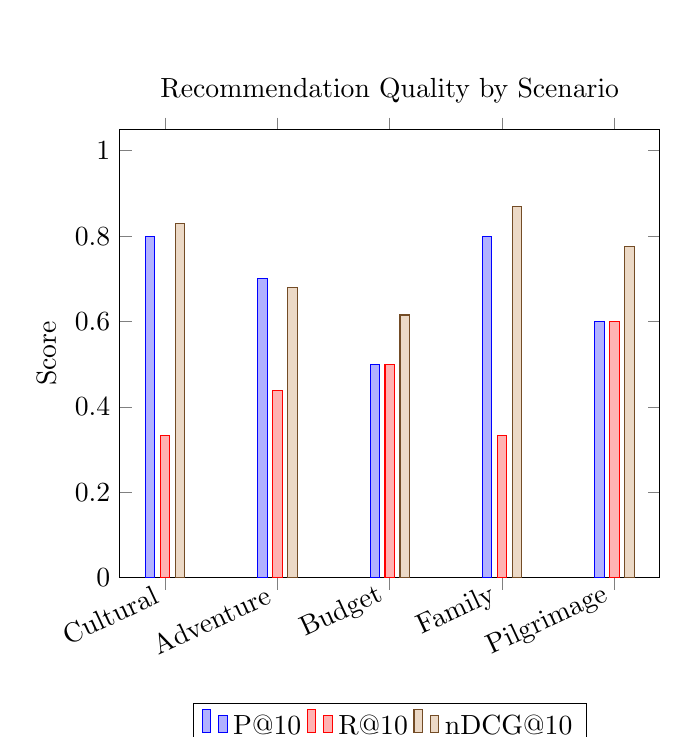
\begin{tikzpicture}
\begin{axis}[
  title=Recommendation Quality by Scenario,
  ylabel=Score,
  ybar,
  bar width=0.12cm,
  symbolic x coords={Cultural,Adventure,Budget,Family,Pilgrimage},
  xtick=data,
  x tick label style={rotate=25,anchor=east},
  legend style={at={(0.5,-0.28)},anchor=north,legend columns=3},
  ymin=0,
  ymax=1.05,
]
\addplot coordinates {(Cultural,0.8000) (Adventure,0.7000) (Budget,0.5000) (Family,0.8000) (Pilgrimage,0.6000)};
\addplot coordinates {(Cultural,0.3333) (Adventure,0.4375) (Budget,0.5000) (Family,0.3333) (Pilgrimage,0.6000)};
\addplot coordinates {(Cultural,0.8305) (Adventure,0.6797) (Budget,0.6152) (Family,0.8701) (Pilgrimage,0.7759)};
\legend{P@10,R@10,nDCG@10}
\end{axis}
\end{tikzpicture}
\caption{Precision, recall, and ranking quality across five tourism scenarios.}
\label{fig:recommendation_metrics}
\end{figure}

The results show that the recommender is strongest for cultural trekking and family-friendly cultural queries. These scenarios achieve Precision@10 of 0.8000 and nDCG@10 above 0.83, suggesting that explicit cultural, family, activity, and season attributes are represented effectively in the dataset and ranking features. Budget relaxation is the weakest scenario, with Precision@10 of 0.5000 and nDCG@10 of 0.6152. This result is understandable because concepts such as peacefulness, relaxation, low cost, and proximity to suitable accommodation are less precisely represented than explicit categories such as pilgrimage or cultural heritage. Improving accommodation pricing, tranquillity features, and budget evidence would therefore be more valuable than simply changing model weights.

MRR is 1.0000 for every scenario, meaning that the first returned destination was relevant in all five tests. This is important for mobile interfaces because users frequently inspect only the first few results. Nevertheless, MRR should not be interpreted as evidence that the complete ranking is perfect. Average Recall@10 is only 0.4408, demonstrating that more than half of all destinations labelled relevant were not recovered in the first ten results. The results therefore support a balanced conclusion: the system is effective at placing at least one useful answer first, but candidate retrieval, attribute completeness, and coverage still require improvement.

\section{Objective Traceability and Evaluation Validity}
\label{sec:validity}

The evaluation evidence can be traced directly to the project objectives. Offline launch, local destination loading, WebP image display, and MBTiles rendering demonstrate that the application preserves its core discovery experience without a network. The routing checks exercise both the online OSRM path and the Haversine fallback. Local chatbot and translation tests examine the offline intelligence objective, while the five recommendation scenarios evaluate semantic retrieval, contextual ranking, and explanation-oriented personalisation. SQLite and Hive behaviour is exercised through saved-place, review, cache, preference, and interaction workflows. Finally, static analysis, backend tests, Flutter tests, APK inspection, and manual offline checks assess the system as an integrated software product rather than as a collection of isolated algorithms.

This traceability also reveals where evidence is weaker. The recommendation metrics show ranking behaviour for defined scenarios, but they do not prove that every tourist would judge relevance in the same way. The relevance labels and scenarios reflect the project's domain assumptions, so changes to labels could change Precision, Recall, nDCG, and MRR. Similarly, a passing offline check proves that a path worked during development; it does not establish long-term reliability across all Android versions, memory constraints, or unusual user actions. The absence of a completed SUS participant study means that ease of use, accessibility, and trust cannot be inferred from functional tests alone.

Several threats to validity therefore remain. Internal validity is affected by the interaction between cached state, device performance, and test order. For example, a warmed recommendation or translation path can appear faster than a first launch. Construct validity is limited because ranking metrics measure relevance and ordering, not whether a recommendation leads to a safe or satisfying visit. External validity is limited by the focus on Gandaki Province, a single Android-oriented implementation, five evaluation scenarios, and development hardware. Ecological validity is also constrained because airplane-mode testing cannot reproduce every rural condition, such as intermittent connectivity, low battery, inaccurate GPS, or rapidly changing road access.

Reproducibility was improved by recording the commands, dataset sizes, asset sizes, metric definitions, scenario-level results, and observed failures. Future evaluation should run the same checks on multiple physical devices, distinguish cold and warm performance, simulate intermittent rather than simply absent connectivity, and recruit domestic and international travelers for task-based testing. Recommendation labels should be reviewed by tourism-domain participants, and online experiments should compare the semantic baseline, contextual reranker, and learned ranking components. These steps would convert the present development evidence into stronger claims about reliability, usability, and real-world tourism value.

\section{Usability Evaluation}
\label{sec:usability}

The System Usability Scale (SUS) was selected as the intended formal usability instrument because it provides a concise ten-item questionnaire that can be applied across different interactive systems \parencite{Brooke1996}. The questionnaire is retained in Table \ref{tbl:sus_items} so that a later participant study can use a consistent instrument. However, a completed formal SUS study with a defensible participant sample was not available at the time of this report. Consequently, no SUS score is reported, and usability conclusions are limited to development feedback, static analysis, widget testing, and observation of the implemented interaction flows.

\begin{table}[h]
\centering
\small
\begin{tabular}{lp{8cm}}
\toprule
\textbf{Item} & \textbf{Statement} \\
\midrule
1 & I think that I would like to use this system frequently. \\
2 & I found the system unnecessarily complex. \\
3 & I thought the system was easy to use. \\
4 & I think that I would need the support of a technical person to use this system. \\
5 & I found the various functions in this system were well integrated. \\
6 & I thought there was too much inconsistency in this system. \\
7 & I would imagine that most people would learn to use this system very quickly. \\
8 & I found the system very cumbersome to use. \\
9 & I felt very confident using the system. \\
10 & I needed to learn a lot of things before I could get going with this system. \\
\bottomrule
\end{tabular}
\caption{System Usability Scale (SUS) items used for usability evaluation.}
\label{tbl:sus_items}
\end{table}

This limitation matters because functional correctness does not guarantee that tourists with different languages, ages, technical confidence, or accessibility needs will find the interface easy to use. A future study should recruit both domestic and international travellers, ask them to complete offline discovery, map, chatbot, translation, save, and recommendation tasks, and combine SUS scores with task completion rates and qualitative interviews.

\section{Comparison with Related Work}
\label{sec:comparison}

\cref{tbl:feature_comparison} compares Paila Nepal with related tourism applications on key features.

\begin{table}[h]
\centering
\small
\begin{tabular}{lcccccc}
\toprule
\textbf{Feature} & \textbf{Google} & \textbf{Trip} & \textbf{OS} & \textbf{Paila} \\
& \textbf{Maps} & \textbf{Advisor} & \textbf{MAnd} & \textbf{Nepal} \\
\midrule
Offline Maps & $\bullet$ & Not supported & $\bullet$ & $\bullet$$\bullet$ \\
Gandaki Focus & Not supported & Not supported & Not supported & $\bullet$$\bullet$ \\
Chatbot Assistance & Not supported & Partial & Not supported & $\bullet$ \\
Destination Recommendations & Partial & $\bullet$ & Not supported & $\bullet$ \\
Offline Routing & Not supported & Not supported & $\bullet$ & $\bullet$ \\
Saved Destinations & $\bullet$ & $\bullet$ & Not supported & $\bullet$ \\
Offline Image Display & Not supported & Not supported & $\bullet$ & $\bullet$$\bullet$ \\
Local NLP Chatbot & Not supported & Not supported & Not supported & $\bullet$ \\
\midrule
\textbf{Offline-First Design} & Not supported & Not supported & Partial & $\bullet$$\bullet$ \\
\textbf{Tourism Specialisation} & Not supported & $\bullet$ & Not supported & $\bullet$$\bullet$ \\
\bottomrule
\end{tabular}
\caption{Feature comparison of tourism applications. Legend: $\bullet$$\bullet$ = full support, $\bullet$ = partial support, Not supported = not supported. Paila Nepal uniquely combines offline-first architecture with rural Gandaki tourism specialisation.}
\label{tbl:feature_comparison}
\end{table}

Paila Nepal's distinctive contributions are:

\begin{enumerate}
\item \textbf{Rural Gandaki Specialisation:} Focuses specifically on rural Gandaki Province destinations, rather than global coverage.

\item \textbf{Truly Offline-First:} All core features function without network connectivity, rather than relying on online connectivity as primary.

\item \textbf{Local Chatbot:} Provides offline conversational tourism assistance without depending on cloud LLMs.

\item \textbf{Integrated Offline Map + Routing + Recommendations:} Combines multiple offline systems into a single cohesive application.

\item \textbf{Tourism-Specific Design:} Includes tourism-relevant attributes (activities, seasons, budget levels, family-friendliness) in destination models.
\end{enumerate}

\section{Limitations and Critical Analysis}
\label{sec:limitations}

Despite the successful implementation of offline-first architecture, several limitations should be acknowledged:

\subsection{Limited Destination Dataset}

The application includes 300 curated Gandaki destinations. While this provides meaningful coverage of major tourism sites, the dataset may not include every lesser-known destination, homestay, or emerging tourism point of interest. Additionally, destination information is static; it does not update in real-time based on community input, seasonal changes, or recent events.

\subsection{Limited Offline Map Zoom}

The offline map MBTiles includes zoom levels 7--12, suitable for regional browsing and destination-level orientation. However, users who zoom beyond level 12 see scaled-up tiles or blank areas if online fallback is disabled. Full street-level mapping would require significantly larger map tiles (potentially 500+ MB), exceeding practical APK distribution constraints.

\subsection{Approximate Offline Routing}

When OSRM is unavailable, the Haversine straight-line route provides direction and distance estimation but not turn-by-turn navigation or road-aware routing. Users must supplement with local knowledge or request directions from residents for final navigation. A fully offline turn-by-turn system would require bundling a complete OpenStreetMap road network, which is beyond current scope.

\subsection{Limited Collaborative Data}

The application includes local ratings/reviews and logs recommendation-related interactions, with queued batch synchronisation to the backend. However, the project has not accumulated a large, representative population of real users. Collaborative scores and learning-to-rank training are therefore constrained by sparse or synthetic interactions. The architecture is ready to learn from future usage, but current evaluation should not imply that the collaborative component has already captured stable population preferences.

\subsection{Language Limitations}

The offline intelligence system supports English, Devanagari Nepali, and romanised Nepali through normalisation, phrasebooks, templates, glossaries, and local retrieval. Nevertheless, it is not equivalent to a large multilingual neural model. Unseen grammar, spelling variation, long-form translation, dialect differences, and culturally specific expressions can still reduce accuracy. The focused performance test also showed a 570 ms warm offline translation result against a 500 ms target, indicating room for optimisation.

\subsection{Device Storage Dependency}

The offline-first design requires bundling significant assets, resulting in a current release APK of approximately 94.97 MB. Older Android devices with limited storage or expensive data plans may find the initial download difficult. This is a reasonable but non-trivial trade-off for comprehensive offline functionality.

\subsection{Lack of Real-Time Data}

The app does not provide real-time information about weather, current events, road conditions, or accommodation availability. This would require continuous backend connectivity to be meaningful.

\section{Societal Impact and Contribution}
\label{sec:impact}

Paila Nepal demonstrates a potential contribution to rural tourism in Nepal:

\subsection{Information Accessibility}

By bundling comprehensive destination information locally, the application increases information accessibility in rural areas where internet connectivity is unreliable. Travelers have access to structured, contextual destination information regardless of network state.

\subsection{Economic Potential}

By increasing digital visibility of rural Gandaki destinations, the application may contribute to tourism demand for rural accommodations, local guides, artisan goods, and cultural experiences. This potential economic benefit accrues primarily to rural communities.

\subsection{Offline-First Design Pattern Contribution}

Paila Nepal demonstrates how offline-first architecture can enhance accessibility in low-connectivity contexts. The design patterns and lessons learned may inform the development of similar applications for other rural tourism regions or resource-constrained contexts globally.

\subsection{Open-Source Potential}

The project (including code, dataset, and architecture) could be open-sourced, allowing other regions to adapt the platform for their local tourism contexts.

\section{Ethical Considerations}
\label{sec:ethics}

Several ethical considerations were addressed during development:

\subsection{Data Privacy}

User location data (if shared) is stored locally on the device. The application does not transmit location data to the backend without explicit user consent. Chatbot interactions remain on-device in offline mode; online LLM requests require user acknowledgement.

\subsection{Accessibility}

The application was designed with accessibility in mind, including readable font sizes, high-contrast colors, and support for standard Android accessibility services. However, some complex features (maps, routing) may benefit from additional accessibility enhancements.

\subsection{Cultural Sensitivity}

Destination descriptions and recommendations respect local culture and traditions. The application emphasizes cultural tourism as meaningful exchange rather than exploitation, and includes warnings about respectful conduct in sacred sites.

\subsection{Fair Attribution}

Destination photographs are sourced from Wikimedia Commons, Wikipedia, and openly-licensed sources. Attribution is provided where appropriate. Destination descriptions are either original or paraphrased from openly-available sources.
\chapter{Challenges and Solutions}
\label{ch:challenges}

\section{Map Tile Format and Compatibility}
\label{sec:ch_tiles}

\textbf{Challenge:} Determining the appropriate map tile format (raster vs. vector) and ensuring compatibility with Flutter map libraries.

\textbf{Solution:} Selected raster PNG tiles in MBTiles format. Raster tiles are directly renderable as images, compatible with \texttt{flutter\_map}, and suitable for offline distribution. Vector tiles (PBF format) would require client-side rendering, adding complexity and library dependencies.

\section{MBTiles Coordinate System}
\label{sec:ch_coords}

\textbf{Challenge:} Resolving coordinate system differences between TMS (Tile Map Service) and XYZ tile coordinate conventions.

\textbf{Solution:} Validated the MBTiles file against both coordinate systems. The Flutter MBTiles provider handles coordinate transformation automatically, so the issue was identified and resolved during testing.

\section{APK Size Management}
\label{sec:ch_apk_size}

\textbf{Challenge:} The combination of the Flutter runtime, destination images, map tiles, and local data resulted in a large APK.

\textbf{Solution:} Optimised images to WebP format, limited map tile zoom levels to 7--12, and limited the destination dataset to Gandaki Province. These choices balanced offline functionality with a release APK size of approximately 94.97 MB.

\section{Offline Routing Fallback}
\label{sec:ch_routing}

\textbf{Challenge:} Providing useful route guidance when online OSRM routing is unavailable.

\textbf{Solution:} Implemented the three-tier routing architecture: cache to OSRM to Haversine fallback. The Haversine fallback provides direction and distance estimation, suitable for initial navigation planning.

\section{Vector vs. Raster Tile Performance}
\label{sec:ch_vector}

\textbf{Challenge:} Vector tiles offer better scalability and smaller file sizes but require client-side rendering.

\textbf{Solution:} Chose raster tiles for simplicity and compatibility with available Flutter libraries. Raster tiles are directly renderable, requiring no client-side vector processing. This trade-off prioritised compatibility over file size.
\chapter{Conclusion}
\label{ch:conclusion}

\section{Summary of Achievements}
\label{sec:summary}

Paila Nepal successfully demonstrates how offline-first mobile architecture can enhance digital accessibility and tourism promotion in rural contexts with limited internet connectivity. The project achieves the following:

\begin{enumerate}
\item \textbf{Offline-First Android Application:} A working Flutter-based Android prototype that preserves destination discovery, map access, fallback route guidance, recommendations, and chatbot assistance without requiring continuous internet connectivity.

\item \textbf{Comprehensive Destination Dataset:} 300 curated Gandaki Province destinations with more than 20 structured and descriptive attributes, 771 accommodation records, and 300 local images.

\item \textbf{Local Asset Integration:} Bundled 300 destination photographs (WebP format), offline map tiles (MBTiles), and chatbot knowledge bases, enabling rich offline experiences.

\item \textbf{Three-Tier Routing System:} Route guidance that gracefully degrades from OSRM road-aware routing to cached routes to Haversine approximation, ensuring users always receive directional guidance.

\item \textbf{Offline Intelligence:} Local multilingual processing, hybrid intent classification, knowledge retrieval, dialogue memory, safety handling, translation, and optional online LLM enhancement.

\item \textbf{Persistent User Data:} SQLite, Hive, and SharedPreferences support for saved destinations, reviews, recommendation caches, route cache, preferences, and queued interactions.

\item \textbf{Explainable Hybrid Recommendations:} SBERT retrieval, collaborative/popularity signals, contextual reranking, cold-start handling, diversity filtering, ML rescoring, and human-readable recommendation reasons.

\item \textbf{Evidence-Based Evaluation:} Five recommendation scenarios, repeatable software checks, explicit reporting of remaining test failures, and a critical analysis of limitations.
\end{enumerate}

\section{Contribution to Knowledge}
\label{sec:contribution}

This project contributes to academic and practical understanding in several areas:

\subsection{Offline-First Architecture for Tourism}

The three-tier routing architecture, tiered data availability, and graceful degradation patterns provide a practical reference for other tourism and low-connectivity applications.

\subsection{Rural Tourism Digitalisation}

The focus on rural Gandaki demonstrates how local content, accessibility, and personalisation can support rural tourism visibility.

\subsection{Mobile Application Design for Low-Connectivity Contexts}

The architecture also illustrates mobile design choices applicable to other regions with unreliable connectivity.

\subsection{Open Dataset and Methodology}

The dataset, knowledge resources, and architecture could be adapted for other regional tourism contexts.

\section{Future Work}
\label{sec:future}

Several directions could extend Paila Nepal:

\subsection{Real User Feedback and Iteration}

Deploying the application to real travelers in Gandaki Province, collecting usage data, and iterating based on user feedback would validate and refine the design.

\subsection{Expanded Destination Dataset}

Incorporating additional destinations beyond the current 300, including homestays, emerging tourism points, and user-contributed information.

\subsection{Full-Length Offline Routing}

Integrating a local road network (e.g., PBF OpenStreetMap extract) to enable turn-by-turn offline navigation without depending on cached routes.

\subsection{Expanded Multilingual Support}

Extending the existing English, Devanagari Nepali, and romanised Nepali resources with broader vocabulary, stronger neural translation, Hindi, Mandarin, and additional tourism-specific language coverage.

\subsection{Community Contributions}

Implementing a backend system for users to submit destination photos, reviews, and information updates, with moderation and synchronisation to the offline app.

\subsection{iOS Support}

Extending the application to iOS using Flutter's cross-platform capabilities.

\subsection{Recommendation Learning from Real Users}

The current system already contains collaborative filtering, semantic embeddings, contextual reranking, a LambdaRank training path, and experimental two-tower components. Future work should therefore focus on collecting consented real-user interactions, evaluating learned ranking against the semantic-only baseline, monitoring fairness and coverage, and retraining safely from representative data.

\subsection{Integration with Nepal Tourism Services}

Partnering with Nepal Tourism Board, accommodation networks, and local tourism operators to integrate booking, weather, verified transport updates, and real-time availability information.

\section{Reflection on Project Outcomes}
\label{sec:reflection}

Paila Nepal addresses the research question by combining bundled destination data and maps with route fallback, local intelligence, offline recommendation assets, and persistent local state. Online-only features, including OSRM road routes and language-model enhancement, deliberately degrade to local alternatives.

However, the project also highlights inherent trade-offs in offline-first design. Bundling significant assets (images, maps) results in a larger APK. Static offline data cannot reflect real-time changes in availability, weather, or events. Offline route computation is approximate compared to road-aware online routing. These trade-offs are intentional and reflect the priorities of accessibility and offline reliability over comprehensiveness and currency.

The evaluation shows both promise and incompleteness. MRR of 1.0000 demonstrates that every tested scenario placed a relevant destination first, while average Recall@10 of 0.4408 shows that relevant destinations are still missed. Static analysis and backend tests pass, but the remaining Flutter widget-test timer and translation performance target demonstrate that further engineering work is required. This balanced outcome is more valuable than claiming production readiness: the project establishes a substantial and testable foundation for future tourism applications and rural digital development initiatives.

\section{Final Remarks}
\label{sec:final}

Paila Nepal demonstrates that tourism technology can respect connectivity constraints by treating offline operation as a core requirement. Its practical patterns, documented limitations, and extensible architecture provide a foundation in practice for future systems serving Gandaki Province and other low-connectivity regions.
\printbibliography[title=References]

\appendix

\chapter{Sample Destination Data}
\label{app:destinations}

\cref{tbl:sample_data} shows the first five destinations from the curated dataset in JSON structure.

\begin{table}[h]
\centering
\small
\begin{tabular}{lp{10cm}}
\toprule
\textbf{Field} & \textbf{Example Value} \\
\midrule
id & destination\_001 \\
name & Ghandruk \\
description & A scenic Gurung village in the Annapurna foothills with traditional stone houses, terraced fields, and warm hospitality... \\
latitude & 28.3956 \\
longitude & 83.8622 \\
category & village \\
activities & ["trekking", "village\_tour", "culture", "nature"] \\
best\_season & ["autumn", "spring"] \\
budget\_level & budget \\
accessibility & moderate \\
adventure\_level & 2 \\
family\_friendly & true \\
cultural\_richness & 8 \\
nature\_score & 7 \\
\bottomrule
\end{tabular}
\caption{Sample destination data structure showing attributes included for each of 300 Gandaki Province destinations.}
\label{tbl:sample_data}
\end{table}

\chapter{API Endpoint Specifications}
\label{app:api_spec}

The FastAPI backend provides the following endpoints:

\begin{table}[h]
\centering
\small
\begin{tabular}{p{4.5cm}p{1.8cm}p{7cm}}
\toprule
\textbf{Endpoint} & \textbf{Method} & \textbf{Purpose} \\
\midrule
/health & GET & Health check \\
/recommend & POST & Hybrid ranked destinations with scores, reasons, cache metadata, and interaction logging \\
/chat & POST & Online chatbot response with local fallback support \\
/chat/offline & POST & Explicit offline rule-based/retrieval response \\
/translate & POST & Supported-pair translation endpoint \\
\path{/auth/register}, \path{/auth/login}, \path{/auth/me} & POST/GET & Authentication and current-user access \\
\path{/destinations}, \path{/destinations/{id}} & GET & Destination catalogue and detail access \\
\path{/destinations/{id}/accommodations} & GET & Accommodation records linked to a destination \\
/similar/\{id\} & GET & Similar-destination semantic retrieval \\
/interactions, /interactions/batch & POST & Single and queued-batch interaction logging \\
/analytics/recommender & GET & Recommender analytics \\
/evaluate/ & POST & Recommendation evaluation metrics \\
/evaluate/train-ranker & POST & Train the LightGBM LambdaRank model \\
/admin/rebuild-index & POST & Rebuild the semantic destination index \\
\bottomrule
\end{tabular}
\end{table}

\chapter{Testing Checklist}
\label{app:testing}

Testing checklist for offline functionality:

\begin{enumerate}
\item Enable airplane mode on test device
\item Launch application and verify successful startup
\item Navigate to home screen and verify no network errors
\item Scroll destination list and verify all 300 destinations load
\item View destination detail screens and verify images display
\item View map screen and verify map tiles render
\item Request route between two destinations and verify Haversine fallback
\item Submit chatbot query and verify offline response
\item Save a destination and verify it persists to SQLite
\item Disable airplane mode and verify app transitions to online mode gracefully
\item Request route and verify OSRM online routing works
\item Clear cache and request previously-used route; verify cache miss and re-computation
\end{enumerate}

\chapter{Database Schema Diagrams}
\label{app:schema}

\begin{figure}[h]
\centering
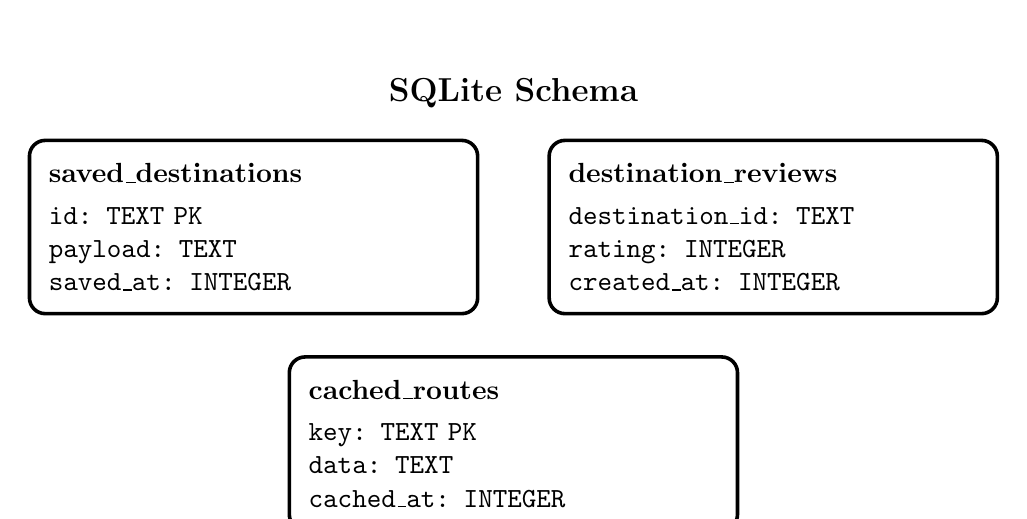
\begin{tikzpicture}[
  schema/.style={draw, rounded corners=2mm, line width=1.3pt, text width=5.2cm, minimum height=2.2cm, align=left, inner sep=7pt}
]
  \node[font=\large\bfseries] at (0,3.2) {SQLite Schema};

  \node[schema] at (-3.3,1.5) {
    \textbf{saved\_destinations}\\[3pt]
    \texttt{id: TEXT PK}\\
    \texttt{payload: TEXT}\\
    \texttt{saved\_at: INTEGER}
  };

  \node[schema] at (3.3,1.5) {
    \textbf{destination\_reviews}\\[3pt]
    \texttt{destination\_id: TEXT}\\
    \texttt{rating: INTEGER}\\
    \texttt{created\_at: INTEGER}
  };

  \node[schema] at (0,-1.25) {
    \textbf{cached\_routes}\\[3pt]
    \texttt{key: TEXT PK}\\
    \texttt{data: TEXT}\\
    \texttt{cached\_at: INTEGER}
  };
\end{tikzpicture}
\caption{Simplified SQLite schema for Paila Nepal. The main application database stores saved destinations and reviews, while a separate SQLite database stores the 30-day route cache. Recommendation caches and pending interactions use Hive.}
\label{fig:db_schema}
\end{figure}

\chapter{System Requirements}
\label{app:requirements}

\textbf{Minimum Device Requirements:}

\begin{itemize}
\item Android 7.0 (API level 24) or higher
\item 2 GB RAM
\item 150 MB free storage (for app + data)
\item GPS and location services
\end{itemize}

\textbf{Recommended Requirements:}

\begin{itemize}
\item Android 10 or higher
\item 4+ GB RAM
\item 200+ MB free storage
\item WiFi + cellular connectivity options
\end{itemize}

\textbf{Development Requirements:}

\begin{itemize}
\item Flutter SDK 3.0.0+
\item Dart 3.x
\item Android Studio 4.1+
\item Android NDK (for native dependencies)
\item Xcode (for iOS development)
\end{itemize}
% Expanded submission evidence. These appendices are intentionally excluded
% from the declared 8,000-word main-body count.

\newcommand{\EvidenceSheet}[7]{%
\clearpage
\section{#1}
\noindent
\begin{tabularx}{\textwidth}{>{\bfseries}p{3.5cm}X}
\toprule
Identifier & #2 \\
Purpose & #3 \\
Preconditions & #4 \\
Procedure or decision & #5 \\
Acceptance evidence & #6 \\
Residual risk & #7 \\
\bottomrule
\end{tabularx}
\vspace{0.8cm}

\noindent\textbf{Traceability note.}
This record connects a stated project requirement to a concrete implementation
or verification activity. It is retained as submission evidence so that the
system can be assessed against observable behaviour rather than feature claims
alone.
}

\chapter{Requirements Catalogue and Traceability}
\label{app:traceability}

This appendix expands the project objectives into assessable requirements.
Priority follows the MoSCoW convention: Must, Should, Could, and Won't for the
current release. The verification column identifies the strongest available
form of evidence.

\begin{longtable}{p{1.4cm}p{8.7cm}p{2.0cm}p{2.2cm}}
\caption{Functional requirements catalogue.}\label{tbl:functional_requirements}\\
\toprule
\textbf{ID} & \textbf{Requirement} & \textbf{Priority} & \textbf{Evidence} \\
\midrule
\endfirsthead
\toprule
\textbf{ID} & \textbf{Requirement} & \textbf{Priority} & \textbf{Evidence} \\
\midrule
\endhead
FR-01 & The application shall launch and expose its core destination catalogue without an active internet connection. & Must & Airplane-mode scenario \\
FR-02 & The application shall load all 300 curated Gandaki Province destination records from bundled assets. & Must & Dataset validation \\
FR-03 & A user shall be able to search and filter destinations by meaningful tourism attributes. & Must & Widget and manual tests \\
FR-04 & A destination detail view shall present descriptive, geographic, seasonal, activity, and image information. & Must & UI inspection \\
FR-05 & The map shall render bundled Gandaki tiles when online tile services are unavailable. & Must & Airplane-mode scenario \\
FR-06 & The routing service shall prefer a cached route, then an online OSRM route, then an offline Haversine fallback. & Must & Routing branch tests \\
FR-07 & Users shall be able to save destinations and retain them between application sessions. & Must & Persistence test \\
FR-08 & Users shall be able to submit and retain local destination reviews. & Should & Persistence test \\
FR-09 & The system shall produce explainable personalized destination recommendations. & Must & Scenario evaluation \\
FR-10 & Recommendation capability shall remain available without the backend. & Must & Offline recommendation test \\
FR-11 & The chatbot shall answer tourism-oriented questions using local intelligence when disconnected. & Must & Intelligence end-to-end test \\
FR-12 & Emergency-like messages shall receive deterministic safety-oriented handling. & Must & Safety scenario test \\
FR-13 & Translation shall support the application's declared English and Nepali travel phrases. & Should & Translation evaluation \\
FR-14 & The application shall queue user interactions locally when the backend is unavailable. & Should & Synchronisation test \\
FR-15 & Queued interactions shall be submitted to the backend after connectivity returns. & Should & Integration scenario \\
FR-16 & The backend shall expose authenticated registration, login, and current user endpoints. & Should & Backend tests \\
FR-17 & The backend shall expose destination and accommodation catalogue endpoints. & Must & API contract test \\
FR-18 & The backend shall expose recommendation, similar-destination, and evaluation endpoints. & Must & API contract test \\
FR-19 & Administrators shall be able to rebuild the semantic destination index. & Could & Endpoint inspection \\
FR-20 & The application shall communicate backend unavailability clearly without preventing local use. & Must & Offline UX inspection \\
\bottomrule
\end{longtable}

\clearpage
\begin{longtable}{p{1.4cm}p{8.7cm}p{2.0cm}p{2.2cm}}
\caption{Non-functional requirements catalogue.}\label{tbl:nonfunctional_requirements}\\
\toprule
\textbf{ID} & \textbf{Requirement} & \textbf{Priority} & \textbf{Evidence} \\
\midrule
\endfirsthead
\toprule
\textbf{ID} & \textbf{Requirement} & \textbf{Priority} & \textbf{Evidence} \\
\midrule
\endhead
NFR-01 & Core discovery, saved data, local recommendations, maps, and local assistance shall tolerate a complete loss of network connectivity. & Must & Airplane-mode suite \\
NFR-02 & The Android release shall remain practical to distribute despite bundled maps, images, and recommendation assets. & Must & APK size inspection \\
NFR-03 & Personal data and authentication secrets shall not be embedded in public application assets. & Must & Configuration review \\
NFR-04 & Backend passwords shall be stored using a one-way password hashing mechanism. & Must & Auth service test \\
NFR-05 & Recommendation results shall include understandable reasons rather than scores alone. & Should & Response inspection \\
NFR-06 & Ranking evaluation shall use repeatable relevance scenarios and standard information-retrieval metrics. & Must & Evaluation script \\
NFR-07 & The app shall use accessible contrast, readable labels, and touch targets suitable for repeated mobile use. & Should & UI inspection \\
NFR-08 & Failures in online enhancement services shall degrade to local capability rather than crash the application. & Must & Failure injection \\
NFR-09 & Local route cache entries shall expire after a defined freshness period. & Should & Cache inspection \\
NFR-10 & Source modules shall retain clear separation between presentation, domain logic, storage, and remote services. & Should & Architecture review \\
NFR-11 & Automated static analysis shall complete without reported Flutter issues. & Must & \texttt{flutter analyze} \\
NFR-12 & Backend automated tests shall pass in the documented environment. & Must & \texttt{pytest} result \\
NFR-13 & The application shall be maintainable through central configuration of its backend base URL. & Should & Configuration review \\
NFR-14 & Dataset fields shall use a consistent schema that can be validated before packaging. & Must & Dataset validation \\
NFR-15 & Safety responses shall be deterministic and shall not depend exclusively on an external language model. & Must & Emergency tests \\
\bottomrule
\end{longtable}

\EvidenceSheet
{Offline Launch and Core Discovery}
{REQ-TRACE-01 / FR-01, FR-02, NFR-01}
{Demonstrate that the application remains useful at initial launch when no network is available.}
{A release build is installed; airplane mode is enabled; bundled assets have not been removed.}
{Launch the app, dismiss onboarding if required, open the home destination feed, perform a destination search, and open a destination detail view. Repeat after force-closing the application.}
{The shell loads without a blocking network error; locally packaged destination content is visible; search and detail navigation remain available; the app can be relaunched.}
{Live events, weather, remote reviews, and newly changed destination information cannot be guaranteed while disconnected.}

\EvidenceSheet
{Bundled Destination Catalogue Integrity}
{REQ-TRACE-02 / FR-02, NFR-14}
{Establish that the packaged catalogue is structurally valid and sufficiently rich for filtering and recommendation.}
{The destination JSON asset is present and the application's destination model is available.}
{Parse the complete asset; check identifier uniqueness; validate coordinates; confirm required text, category, activity, season, budget, accessibility, family, culture, nature, and image fields; report malformed records.}
{All 300 intended destination records load through the real model mapping and can be used by discovery and recommendation services.}
{Curated data can become stale; a future release requires a governed update and validation process.}

\EvidenceSheet
{Offline Map Availability}
{REQ-TRACE-03 / FR-05, NFR-01}
{Confirm that map exploration does not disappear when an online tile provider cannot be reached.}
{The Gandaki MBTiles asset is packaged; location permission is granted or a known map location is selected.}
{Enable airplane mode, open the map, pan across Pokhara and surrounding Gandaki areas, change supported zoom levels, and reopen the map after restarting the app.}
{Raster tiles render from the bundled database for the declared coverage and zoom range without a tile-network dependency.}
{Coverage is deliberately bounded; street-level tiles outside the packaged region or zoom range are unavailable.}

\EvidenceSheet
{Three-Tier Route Resolution}
{REQ-TRACE-04 / FR-06, NFR-08, NFR-09}
{Verify deterministic routing behaviour across cached, online, and fully disconnected states.}
{Two valid coordinates are selected and the route cache can be inspected or cleared.}
{Request a route once online, repeat to exercise the cache, then clear the relevant entry and request the route in airplane mode. Compare route source, distance, and presentation.}
{The first eligible online request uses OSRM, the repeated request can use the SQLite cache, and the disconnected cache miss produces a Haversine fallback instead of a crash.}
{The Haversine line is an estimate and must not be presented as road-aware turn-by-turn navigation.}

\EvidenceSheet
{Persistent Saved Destinations and Reviews}
{REQ-TRACE-05 / FR-07, FR-08}
{Confirm that user-created local state survives navigation and process restarts.}
{At least one destination is available; application storage has not been manually cleared.}
{Save a destination, submit a local review, navigate away, force-close the app, relaunch, and inspect saved and reviewed content. Then remove the saved item and confirm the change persists.}
{SQLite-backed saved and review state remains consistent across sessions and reflects create and delete actions.}
{Device uninstall or storage clearing removes local-only state unless a future synchronisation feature has uploaded it.}

\EvidenceSheet
{Offline Recommendation Continuity}
{REQ-TRACE-06 / FR-09, FR-10, NFR-05}
{Demonstrate that personalization is not exclusively dependent on the FastAPI service.}
{Destination assets and local recommendation resources are packaged; user preferences can be supplied.}
{Generate recommendations online, disable connectivity, change a preference or context, and generate recommendations again. Inspect ordering, reasons, and absence of blocking errors.}
{The offline pipeline returns ranked destinations with human-readable reasons and uses locally available semantic and contextual signals.}
{Offline ranking does not have access to fresh cross-user interaction data or newly trained backend models.}

\EvidenceSheet
{Local Tourism Assistance and Safety}
{REQ-TRACE-07 / FR-11, FR-12, NFR-15}
{Verify that local intelligence can answer supported tourism questions and prioritise emergency handling.}
{Offline knowledge assets and intelligence services are initialized; network connectivity is disabled.}
{Ask for a destination suggestion, a practical travel phrase, a follow-up question requiring context, and an emergency-style message. Inspect response mode and safety content.}
{Supported tourism queries receive local retrieval or template responses; conversation state is retained; emergency content is handled by deterministic safety logic.}
{The assistant is not a substitute for emergency services, medical advice, or verified real-time trail conditions.}

\EvidenceSheet
{Backend Failure Degradation}
{REQ-TRACE-08 / FR-20, NFR-08, NFR-13}
{Confirm that a backend outage is visible but does not disable local application features.}
{The app is configured with a deliberately unreachable backend URL while local assets remain intact.}
{Launch the app, trigger a backend-enhanced action, inspect the user-facing state, then continue to discovery, map, saved items, local recommendations, and local chatbot functions.}
{The application communicates that online services are unavailable and continues to expose its offline-capable workflows.}
{Remote-only capabilities such as authentication, fresh analytics, and online model responses remain unavailable until connectivity and backend health recover.}

\chapter{Data Dictionary and Dataset Evidence}
\label{app:data_dictionary}

The recommendation and discovery experience depends on consistent structured
data. The following dictionary documents the principal destination fields used
across Flutter and FastAPI components.

\begin{longtable}{p{3.2cm}p{2.2cm}p{6.1cm}p{2.5cm}}
\caption{Destination data dictionary.}\label{tbl:data_dictionary}\\
\toprule
\textbf{Field} & \textbf{Type} & \textbf{Meaning and use} & \textbf{Validation} \\
\midrule
\endfirsthead
\toprule
\textbf{Field} & \textbf{Type} & \textbf{Meaning and use} & \textbf{Validation} \\
\midrule
\endhead
\texttt{id} & string & Stable destination key used by UI, persistence, routes, interactions, and recommendation outputs. & Required; unique \\
\texttt{name} & string & Human-readable destination name displayed throughout the application. & Required; non-empty \\
\texttt{description} & string & Curated descriptive content for details, retrieval, and semantic embedding. & Required; non-empty \\
\texttt{latitude} & number & Geographic latitude used by maps, distance features, and routing. & -90 to 90 \\
\texttt{longitude} & number & Geographic longitude used by maps, distance features, and routing. & -180 to 180 \\
\texttt{category} & string & Primary tourism category such as village, lake, viewpoint, temple, or trek. & Controlled value \\
\texttt{activities} & list & Supported experiences such as trekking, culture, nature, photography, or pilgrimage. & Non-empty list \\
\texttt{best\_season} & list & Seasons in which the destination is most suitable. & Controlled values \\
\texttt{budget\_level} & string & Relative cost category used by filters and contextual scoring. & Controlled value \\
\texttt{accessibility} & string & Relative access difficulty used in suitability filtering and explanations. & Controlled value \\
\texttt{adventure\_\allowbreak level} & integer & Ordinal indicator of desired physical/adventure intensity. & Bounded scale \\
\texttt{family\_\allowbreak friendly} & boolean & Indicates suitability for family-oriented discovery scenarios. & Boolean \\
\texttt{cultural\_\allowbreak richness} & number & Relative cultural value used in filters and ranking features. & Bounded scale \\
\texttt{nature\_score} & number & Relative natural-attraction value used in filters and ranking features. & Bounded scale \\
\texttt{tags} & list & Additional searchable and semantically useful descriptive labels. & Normalised strings \\
\texttt{image} & string & Local or resolvable image reference used by cards and detail presentation. & Asset existence \\
\texttt{sbert\_text} & string & Prepared semantic text combining meaningful destination attributes. & Non-empty text \\
\texttt{province} & string & Administrative region used to constrain and describe coverage. & Gandaki scope \\
\bottomrule
\end{longtable}

\EvidenceSheet
{Dataset Identity and Uniqueness}
{DATA-EVIDENCE-01}
{Prevent ambiguous persistence, interaction, and recommendation references.}
{The complete destination asset is available to a validation script or model loader.}
{Collect every destination identifier and name; report empty values, duplicate identifiers, and suspicious duplicate normalized names; verify that referenced identifiers remain stable between app and backend assets.}
{Every packaged destination has one stable unique identifier and a usable display name.}
{Name changes and future record merges require migration rules so saved items and interactions remain associated correctly.}

\EvidenceSheet
{Geographic Validity}
{DATA-EVIDENCE-02}
{Ensure that destination points can be rendered, measured, and routed without invalid coordinates.}
{All records have been parsed into numeric latitude and longitude values.}
{Check global coordinate bounds, inspect whether points fall within the intended Nepal/Gandaki coverage, and plot outliers for manual review.}
{All intended destinations produce valid map points and no record silently defaults to an unrelated coordinate.}
{A valid coordinate does not guarantee a safe or publicly accessible arrival point; field verification remains necessary.}

\EvidenceSheet
{Semantic Retrieval Readiness}
{DATA-EVIDENCE-03}
{Confirm that recommendation and chatbot retrieval operate on informative text rather than destination names alone.}
{Each record exposes description, category, activity, tag, and prepared semantic text fields.}
{Inspect representative records across categories; compare source attributes with prepared semantic text; check for empty or duplicated semantic content; verify embedding-index alignment with identifiers.}
{Semantic records contain enough distinct tourism context to support similarity search and scenario-oriented ranking.}
{Curated descriptions may reflect author bias and can underrepresent less documented communities.}

\EvidenceSheet
{Local Media Integrity}
{DATA-EVIDENCE-04}
{Verify that offline destination presentation can resolve packaged images reliably.}
{The Flutter asset manifest and local image directory are available.}
{Resolve each destination image reference, identify missing or duplicate assets, open a sample across image sizes, and inspect card/detail fallback behaviour.}
{Intended local image references resolve and missing media does not crash a destination card or details screen.}
{Image licensing, accessibility text, and future content updates require an explicit governance process.}

\EvidenceSheet
{Accommodation Relationship Integrity}
{DATA-EVIDENCE-05}
{Confirm that accommodation records can be associated with their destination context.}
{The accommodation dataset and destination identifier set are available.}
{Validate accommodation identifiers, destination foreign-key references, coordinates, names, types, price data, and duplicated records; inspect destinations with zero and many linked accommodations.}
{Each of the 771 intended accommodation records is parseable and every declared destination relationship resolves.}
{Availability and prices are not real-time and must be labelled accordingly in future booking-oriented releases.}

\chapter{Detailed API Contract Catalogue}
\label{app:api_contracts}

Each contract sheet records the behaviour expected by the Flutter client and by
administrative or evaluation tooling. Exact payloads remain versioned by the
backend implementation; the sheets focus on externally observable obligations.

\EvidenceSheet
{Health Check Contract}
{API-01 / \texttt{GET /health}}
{Provide a low-cost signal that the FastAPI process is reachable before online enhancement is attempted.}
{The backend process has started and its configured port is reachable.}
{Send an unauthenticated GET request; inspect status code and response body; repeat while a downstream optional model provider is unavailable.}
{The endpoint returns a successful service-health response without requiring user credentials or an external model provider.}
{Process health alone does not prove that every optional dependency or data source is healthy.}

\EvidenceSheet
{Destination Collection Contract}
{API-02 / \texttt{GET /destinations}}
{Expose the destination catalogue for online consumers and consistency checks.}
{The backend destination repository has loaded its dataset.}
{Request the collection; inspect record count, identifiers, names, coordinates, and pagination or limit behaviour if configured.}
{The response is valid JSON, uses stable identifiers, and exposes fields compatible with the client destination model.}
{Large future datasets require explicit pagination and version-aware client handling.}

\EvidenceSheet
{Destination Detail and Accommodation Contract}
{API-03 / \texttt{GET /destinations/\{id\}} and accommodation route}
{Expose one destination and its linked accommodation context.}
{A valid destination identifier and an invalid test identifier are available.}
{Request a valid detail record, request its accommodations, then request a missing identifier and inspect error semantics.}
{Valid requests return the intended record and relationships; missing identifiers return a controlled not-found response rather than a server error.}
{Accommodation data remains informational unless integrated with a verified availability provider.}

\EvidenceSheet
{Recommendation Contract}
{API-04 / \texttt{POST /recommend}}
{Return ranked and explainable destination suggestions for a supplied user and context.}
{The destination index and recommendation service are initialized; a valid request payload is available.}
{Submit a cold-start request, a preference-rich request, and a request with contextual attributes; inspect ordering, scores, reasons, metadata, and repeatability.}
{The endpoint returns a bounded ranked list with stable identifiers, interpretable reasons, and metadata sufficient for client presentation and analysis.}
{Sparse or synthetic interactions limit confidence in collaborative and learned ranking signals.}

\EvidenceSheet
{Similar Destination Contract}
{API-05 / \texttt{GET /similar/\{id\}}}
{Support related-destination discovery using semantic similarity.}
{A valid indexed destination identifier is available.}
{Request similar destinations, verify that the source destination is excluded, inspect similarity ordering, and test a missing identifier.}
{The response contains valid alternatives with scores or ordering consistent with the semantic index.}
{Semantic similarity can reinforce catalogue-description bias and does not automatically provide diversity.}

\EvidenceSheet
{Interaction Logging Contract}
{API-06 / \texttt{POST /interactions} and \texttt{/interactions/batch}}
{Accept behavioural events used for analytics and future recommendation improvement.}
{The interaction repository is writable and test user/destination identifiers are available.}
{Submit a single event, submit a mixed batch, inspect accepted counts, test validation failures, and verify repository persistence.}
{Valid events are stored once with required context; invalid events receive controlled validation responses; batch results expose partial-failure semantics.}
{Interaction collection requires consent, retention controls, and protection against event duplication or manipulation.}

\EvidenceSheet
{Chat Contract}
{API-07 / \texttt{POST /chat}}
{Provide online-enhanced tourism assistance while preserving controlled fallback behaviour.}
{The chat route is registered; at least one provider or fallback service is available.}
{Send representative discovery, route, translation, follow-up, unsupported, and provider-failure prompts; inspect response source and safety handling.}
{The endpoint returns a structured response and does not expose provider exceptions directly to the client.}
{External provider content can be inaccurate; the client must preserve safety disclaimers and local fallback.}

\EvidenceSheet
{Offline Chat Contract}
{API-08 / \texttt{POST /chat/offline}}
{Expose the backend's deterministic offline-oriented retrieval response for explicit testing and fallback use.}
{Offline chat data and service initialization have completed.}
{Submit supported and unsupported tourism prompts and inspect intent, response text, and destination references.}
{The endpoint responds without calling a cloud language model and returns controlled content for supported local knowledge.}
{The available response range is narrower than generative online assistance.}

\EvidenceSheet
{Translation Contract}
{API-09 / \texttt{POST /translate}}
{Provide supported travel translation with explicit language-pair and failure semantics.}
{Translation resources are initialized and a supported-pair matrix is documented.}
{Submit representative supported phrases, mixed-case input, romanised Nepali, an unsupported pair, and empty or excessive input.}
{Supported requests return structured translated text and language metadata; invalid requests receive controlled validation errors.}
{Coverage remains domain-specific and should not be represented as general professional translation.}

\EvidenceSheet
{Authentication Contract}
{API-10 / registration, login, and current-user routes}
{Provide identity for optional synchronized and personalized online capability.}
{The authentication repository and secret configuration are available.}
{Register a new account, reject duplicate or invalid input, login with correct and incorrect credentials, then access the current-user route with valid, expired, and missing tokens.}
{Passwords are not returned or stored in plain text; successful login returns a usable token; protected access rejects invalid credentials.}
{Authentication security also depends on deployment TLS, secret rotation, rate limiting, and production monitoring.}

\chapter{Verification Test Catalogue}
\label{app:test_catalogue}

The following cases describe repeatable acceptance and regression checks. They
supplement automated unit and widget tests with integrated offline-first
scenarios that cross storage, presentation, networking, and intelligence
boundaries.

\EvidenceSheet
{Cold Offline Startup Test}
{TEST-ACC-01}
{Test the most important failure condition: no connection at the start of a session.}
{Install the release build; clear recent tasks; enable airplane mode before launching.}
{Launch, complete or skip onboarding, open home, search, details, map, saved items, recommendations, chatbot, and translation in sequence.}
{Core local screens remain reachable; no infinite loading state or uncaught network exception prevents continued use.}
{Some screens can correctly show that optional online enhancement is unavailable.}

\EvidenceSheet
{Warm Online-to-Offline Transition Test}
{TEST-ACC-02}
{Check graceful degradation when connectivity disappears during active use.}
{The application is open and the backend is initially reachable.}
{Load online recommendations and a road route, disable connectivity, repeat both actions, then open local content and send a chatbot query.}
{Cached or local alternatives are used where designed; the state change is communicated without a crash.}
{An in-flight remote request may take until its configured timeout before fallback occurs.}

\EvidenceSheet
{Offline-to-Online Recovery Test}
{TEST-ACC-03}
{Check that the app recovers online capability without requiring reinstallation or data loss.}
{The app has been used offline and contains queued interactions.}
{Restore connectivity, trigger health checking or retry, request an online route, and observe interaction synchronization.}
{Online capability returns; queued events can be submitted; local saved state and caches remain intact.}
{Recovery timing depends on platform connectivity signals and backend availability.}

\EvidenceSheet
{Route Cache Precedence Test}
{TEST-ACC-04}
{Prove that an eligible cached route takes precedence and avoids unnecessary network use.}
{A known OSRM route has been cached and remains within the configured freshness period.}
{Request the identical coordinate pair with network available and inspect route source and outgoing traffic; repeat after expiry or cache removal.}
{The fresh cache serves the repeat request; expired or absent entries allow later routing tiers to execute.}
{Coordinate rounding and cache-key design can affect hit rate for nearly identical points.}

\EvidenceSheet
{Haversine Fallback Test}
{TEST-ACC-05}
{Confirm that a disconnected cache miss still returns a useful directional estimate.}
{No relevant route is cached and the device is offline.}
{Request a route between two valid destinations and compare reported straight-line distance with an independently calculated Haversine value.}
{A clearly identified fallback route is returned with plausible distance and without turn-by-turn claims.}
{Terrain, roads, bridges, closures, and walking feasibility are not represented by the fallback line.}

\EvidenceSheet
{Recommendation Scenario Evaluation Test}
{TEST-REC-01}
{Measure ranked retrieval quality against the report's five defined tourism scenarios.}
{Scenario queries, relevance sets, and the candidate destination catalogue are fixed for the run.}
{Generate top-ten rankings for every scenario and calculate Precision@10, Recall@10, nDCG@10, and MRR using the same relevance judgments.}
{Metric calculation is reproducible and results can be compared with the documented hybrid recommender values.}
{Five scenarios are useful for project evaluation but insufficient to establish population-level effectiveness.}

\EvidenceSheet
{Recommendation Explanation Test}
{TEST-REC-02}
{Verify that recommendation reasons correspond to actual ranking features and destination attributes.}
{A set of recommendations with score components and destination records is available.}
{Inspect reasons for season, activity, budget, distance, culture, nature, popularity, and similar-item signals; compare each statement with source attributes.}
{Reasons are understandable and do not claim attributes that the destination record or ranking path does not support.}
{Simplified explanations cannot fully describe every interaction within a learned ranking model.}

\EvidenceSheet
{Cold-Start Recommendation Test}
{TEST-REC-03}
{Confirm that a new user receives useful, diverse suggestions without an interaction history.}
{Use a new anonymous identifier or clear local recommendation history.}
{Request recommendations with no preferences, then with onboarding preferences; inspect relevance, diversity, and explanation changes.}
{The system supplies reasonable defaults and responds to explicit preferences without requiring collaborative history.}
{Popularity-based defaults can overexpose already prominent destinations.}

\EvidenceSheet
{Emergency Detection Test}
{TEST-AI-01}
{Verify deterministic priority handling of messages that indicate immediate danger or need for assistance.}
{The local intelligence pipeline is initialized and external AI providers are disabled.}
{Submit representative emergency, injury, lost-person, and benign messages in supported language forms; inspect detection and response precedence.}
{Emergency-like messages trigger the safety layer before normal tourism recommendation generation; benign queries avoid false emergency escalation.}
{Language variation and ambiguous messages require continuing review with domain experts.}

\EvidenceSheet
{Dialogue Continuity Test}
{TEST-AI-02}
{Check that follow-up questions can use recent conversation context.}
{Start a fresh conversation and ask for a destination recommendation with explicit constraints.}
{Send follow-ups that omit the destination name but refer to cost, route, season, and alternatives; then reset the conversation.}
{Relevant recent slots and entities are retained before reset and are not incorrectly reused after reset.}
{Long conversations and topic changes can still create ambiguity requiring clarification.}

\EvidenceSheet
{Translation Coverage Test}
{TEST-AI-03}
{Evaluate supported travel phrases, normalization, and controlled fallback behaviour.}
{The local glossary, phrasebook, templates, and available online adapter are known.}
{Test exact phrases, punctuation and case variants, romanised Nepali, Devanagari input, unsupported text, and provider unavailability.}
{Supported local phrases translate consistently; response metadata distinguishes translation source or fallback state.}
{General prose, specialist terminology, and dialect variation remain outside validated coverage.}

\EvidenceSheet
{Static Analysis and Automated Regression Test}
{TEST-ENG-01}
{Provide repeatable engineering-quality evidence for Flutter and backend components.}
{Dependencies are installed in the documented environments.}
{Run Flutter static analysis, focused intelligence and recommendation tests, backend pytest, and relevant widget tests; retain command, date, environment, and outcome.}
{Static analysis and focused suites produce a clear pass/fail signal; known failures are documented rather than concealed.}
{Environment-specific timing and golden-image rendering can differ across machines and SDK versions.}

\chapter{User Manual and Operational Workflows}
\label{app:user_manual}

This manual describes the intended end-user workflows. Screen names may evolve,
but the operational sequence and offline expectations remain part of the
project's acceptance baseline.

\EvidenceSheet
{First Launch and Onboarding}
{USER-01}
{Help a first-time traveler configure useful preferences without blocking immediate exploration.}
{The application is installed and launched for the first time.}
{Review onboarding, choose available preferences where offered, grant only required permissions, and continue to the main dashboard.}
{The user reaches the application shell; declared preferences can influence discovery and recommendation; denied optional permissions do not prevent catalogue browsing.}
{Location-dependent convenience is reduced when location permission is denied.}

\EvidenceSheet
{Browse and Search Destinations}
{USER-02}
{Find relevant destinations from the bundled Gandaki catalogue.}
{The home or discovery screen is open.}
{Scroll destination content, enter a search term, apply available filters, clear the query, and open a result.}
{Results respond to the query and filters; destination cards remain readable; clearing controls restores broader discovery.}
{Search quality depends on the vocabulary represented in the curated dataset.}

\EvidenceSheet
{Read Destination Details}
{USER-03}
{Inspect practical and descriptive information before deciding to travel.}
{A destination card or recommendation has been selected.}
{Review description, images, category, activities, season, budget, accessibility, location, and available accommodation context; follow map or save actions.}
{Information is presented consistently and available local assets remain visible without a connection.}
{Static descriptions cannot replace local safety advice or real-time access information.}

\EvidenceSheet
{Save and Review a Destination}
{USER-04}
{Retain personal travel interests and feedback locally.}
{A destination detail view is open and local storage is available.}
{Toggle the saved state, locate the destination in saved content, create or update a review, restart the app, and inspect persistence.}
{Saved and review state remains available after restart and can be intentionally changed or removed.}
{Local-only state is lost if application storage is cleared or the app is uninstalled.}

\EvidenceSheet
{Explore the Offline Map}
{USER-05}
{Use geographic context in places with unreliable mobile data.}
{The map screen is available and the bundled tile database is packaged.}
{Open the map, move to a known Gandaki area, pan and zoom within supported coverage, select a destination marker, and inspect the details action.}
{The map remains usable within packaged coverage and destination points connect to discovery workflows.}
{The bundled raster map is a snapshot and does not show live closures or every street-level detail.}

\EvidenceSheet
{Request Directions}
{USER-06}
{Obtain the best available route representation for the current connectivity state.}
{Origin and destination coordinates are available; location permission is granted if current position is used.}
{Request a route; inspect whether it is cached, road-aware online, or straight-line fallback; review distance and any warning; repeat offline.}
{The route source is understandable and the app does not imply road guidance when only a Haversine estimate is available.}
{Users must verify local conditions and should not rely solely on the fallback for safety-critical navigation.}

\EvidenceSheet
{Receive Personalized Recommendations}
{USER-07}
{Discover destinations that align with interests, season, budget, accessibility, and context.}
{The recommendation view is open and local destination data has loaded.}
{Provide or change available preference controls, request recommendations, read explanation text, open a suggested destination, and repeat without connectivity.}
{Ranked results update meaningfully and expose reasons that help the user judge suitability.}
{Recommendations assist discovery but do not guarantee satisfaction, safety, or availability.}

\EvidenceSheet
{Use the Tourism Chatbot}
{USER-08}
{Ask natural-language tourism questions and receive the best available local or online-enhanced response.}
{The chatbot screen is open.}
{Ask a specific question, use a follow-up, request an alternative, disconnect the network, and ask another supported local question.}
{The conversation remains usable; response state distinguishes fallback where appropriate; local questions continue to receive controlled assistance.}
{Generated or retrieved answers can be incomplete and should be verified for high-stakes decisions.}

\EvidenceSheet
{Translate a Travel Phrase}
{USER-09}
{Support practical communication using available English and Nepali resources.}
{The translation screen is open and source/target languages can be selected.}
{Enter a supported travel phrase, translate it, swap direction where supported, test romanised or Devanagari input, and repeat offline.}
{Supported content produces a readable result and offline resources remain available for their declared coverage.}
{The feature is not a certified interpreter and should not be relied on for legal or medical communication.}

\EvidenceSheet
{Recognise Offline and Recovery States}
{USER-10}
{Help users understand which capabilities remain local and which require the network.}
{The application is running and connectivity can be toggled.}
{Disable the network, observe messaging while using local features, attempt an online enhancement, restore connectivity, and retry.}
{The application communicates backend or connectivity loss without hiding local capability and recovers online actions when service returns.}
{Connectivity indicators can lag behind the actual reachability of a particular external service.}

\chapter{Deployment, Configuration, and Troubleshooting}
\label{app:operations}

\EvidenceSheet
{Flutter Development Setup}
{OPS-01}
{Provide a repeatable setup path for application development and verification.}
{Flutter, Dart, Android tooling, and a supported device or emulator are available.}
{Open the \texttt{app} directory, obtain dependencies, inspect environment configuration, run static analysis and focused tests, then launch a debug build.}
{Dependencies resolve, analysis completes, tests provide a clear result, and the app launches against the intended local or remote backend configuration.}
{SDK and plugin upgrades can change build behaviour; versions should be recorded for reproducibility.}

\EvidenceSheet
{Backend Development Setup}
{OPS-02}
{Provide a repeatable FastAPI setup for recommendation, chat, authentication, and analytics development.}
{A supported Python environment and project dependencies are available.}
{Configure environment variables, initialize required data, run backend tests, start the API server, and request the health endpoint.}
{Tests and health checking provide a clear operational signal and registered routes are visible through FastAPI documentation.}
{Optional provider keys and production databases require separate secure configuration.}

\EvidenceSheet
{Backend URL and Environment Switching}
{OPS-03}
{Avoid scattered host literals and support emulator, device, and deployed environments.}
{The central application backend configuration is available.}
{Set the intended backend environment or base URL, launch the app, inspect the health request, and verify that feature services derive their URIs from the central configuration.}
{Runtime requests use the selected central base URL and backend failure is surfaced through the intended offline UX.}
{Physical devices, emulators, and remote deployments have different network addressing and firewall constraints.}

\EvidenceSheet
{Android Release Build and Asset Verification}
{OPS-04}
{Produce a distributable package containing the offline assets required by the project.}
{Release signing and Flutter Android tooling are configured.}
{Build the release APK, inspect size, install it on a clean device, enable airplane mode, and verify destination data, images, MBTiles, and local intelligence assets.}
{The release installs and core offline workflows operate without relying on development-machine files.}
{Bundled assets increase download size and must be revalidated after asset-manifest changes.}

\EvidenceSheet
{Operational Troubleshooting Guide}
{OPS-05}
{Provide a systematic response to common failures without masking data loss or unsafe behaviour.}
{Logs, app settings, and health endpoints are available to the developer or tester.}
{For startup failure, inspect asset parsing and storage initialization; for backend failure, inspect base URL and health; for blank maps, inspect MBTiles packaging; for stale routes, inspect cache age; for AI failure, inspect local initialization before provider status.}
{Troubleshooting isolates the affected tier and preserves local functionality wherever possible.}
{Clearing application data is a last resort because it removes saved local state and can hide the original fault.}

\chapter{Architecture Decision Records}
\label{app:adrs}

\EvidenceSheet
{Use Flutter for the Mobile Client}
{ADR-01 / Accepted}
{Deliver a maintainable Android application with a consistent component model and future cross-platform potential.}
{The project requires a rich mobile interface, local storage, maps, and broad plugin support.}
{Adopt Flutter and Dart; structure features around presentation, domain models, and services; use platform integrations only where required.}
{The implemented client provides the intended screens, local data access, maps, and testable Dart services from one codebase.}
{Plugin quality and native build complexity can affect platform-specific behaviour.}

\EvidenceSheet
{Treat Offline Operation as the Default Architecture}
{ADR-02 / Accepted}
{Preserve useful travel support in the low-connectivity conditions central to the research problem.}
{Core catalogue, media, maps, routing fallback, storage, recommendations, and assistance can be packaged or computed locally.}
{Design local capability first and layer remote enhancement behind reachability checks, timeouts, caching, queues, and controlled fallback.}
{The application remains useful during backend or network loss and does not place every workflow behind authentication.}
{Offline assets are static and increase package size; synchronization requires careful conflict and freshness handling.}

\EvidenceSheet
{Use FastAPI for Online Enhancement Services}
{ADR-03 / Accepted}
{Expose typed Python services for recommendation, semantic search, evaluation, chat, analytics, and authentication.}
{The recommendation and NLP ecosystem is primarily Python-based and benefits from automatic API documentation.}
{Implement versioned route modules and application services in FastAPI; keep offline-critical capability in Flutter.}
{Online services can evolve independently while the client preserves local fallback.}
{A production deployment still requires TLS, observability, scaling, rate limiting, and secret management.}

\EvidenceSheet
{Combine SQLite, Hive, and SharedPreferences}
{ADR-04 / Accepted}
{Match local persistence mechanisms to relational records, high-frequency cached objects, queues, and lightweight settings.}
{Saved destinations, reviews, routes, recommendation caches, interactions, and preferences have different access patterns.}
{Use SQLite for relational saved/review/route data, Hive for recommendation cache and pending interactions, and SharedPreferences for small settings.}
{Each local data category has a storage mechanism appropriate to its structure and lifecycle.}
{Multiple stores increase migration, backup, and debugging complexity.}

\EvidenceSheet
{Bundle MBTiles for Offline Map Coverage}
{ADR-05 / Accepted}
{Ensure that geographic context remains available without runtime tile downloads.}
{A bounded Gandaki coverage area and practical zoom range are acceptable for the project.}
{Package a local raster MBTiles database and use online services only as optional enhancement.}
{The app renders the intended Gandaki map region in airplane mode.}
{Higher zoom levels and expanded coverage would substantially increase package size.}

\EvidenceSheet
{Use Cache, OSRM, then Haversine for Routing}
{ADR-06 / Accepted}
{Provide the best available route response while guaranteeing a disconnected fallback.}
{Road-aware offline routing data is too large or complex for the current scope.}
{Resolve routes through a fresh SQLite cache, then online OSRM, then a clearly identified straight-line Haversine approximation.}
{Repeated routes are efficient, online routes can be road-aware, and disconnected cache misses still return useful orientation.}
{The fallback must never be confused with safe road or trail instructions.}

\EvidenceSheet
{Hybrid Explainable Recommendation Pipeline}
{ADR-07 / Accepted}
{Balance semantic relevance, context, interaction evidence, diversity, and understandable user-facing reasons.}
{The catalogue contains rich text and attributes, while real-user interaction volume remains limited.}
{Combine semantic candidates, collaborative/popularity signals, contextual reranking, optional learned rescoring, diversity control, and explanation generation.}
{Scenario evaluation demonstrates strong first-result placement and exposes measurable recall limitations.}
{Learned and collaborative components require representative consented usage data before strong production claims.}

\EvidenceSheet
{Keep Deterministic Local Safety and Intelligence}
{ADR-08 / Accepted}
{Avoid making tourism assistance and emergency handling wholly dependent on a network or generative provider.}
{Local language processing, retrieval, dialogue state, phrase resources, and emergency rules can run on-device.}
{Run deterministic safety handling and local intelligence for every relevant message, using online language models only as an optional enhancement.}
{Supported queries and emergency-like messages retain controlled handling during provider or network failure.}
{Local coverage is finite and requires continued multilingual testing and expert review.}

\chapter{Selected Implementation Listings}
\label{app:listings}

The following listings are drawn directly from the implemented project. They
are included as technical evidence rather than as a claim that every source
file belongs in the dissertation. Line numbers support discussion and review.

\clearpage
\section{FastAPI Recommendation Route}
\lstinputlisting[
  language=Python,
  numbers=left,
  basicstyle=\ttfamily\scriptsize,
  caption={Implemented recommendation API route.}
]{../backend/api/v1/recommend.py}

\clearpage
\section{Backend Recommendation Application Service}
\lstinputlisting[
  language=Python,
  numbers=left,
  basicstyle=\ttfamily\scriptsize,
  caption={Implemented hybrid recommendation application service.}
]{../backend/application/services/recommendation_service.py}

\clearpage
\section{Backend Contextual Reranker Excerpt}
\lstinputlisting[
  language=Python,
  firstline=1,
  lastline=260,
  numbers=left,
  basicstyle=\ttfamily\scriptsize,
  caption={Selected contextual reranking implementation.}
]{../backend/infrastructure/ml/contextual_reranker.py}

\clearpage
\section{Flutter Routing Service}
\lstinputlisting[
  numbers=left,
  basicstyle=\ttfamily\scriptsize,
  caption={Implemented Flutter routing service with fallback tiers.}
]{../app/lib/core/navigation/routing_service.dart}

\clearpage
\section{Offline Semantic Encoder}
\lstinputlisting[
  numbers=left,
  basicstyle=\ttfamily\scriptsize,
  caption={Implemented offline semantic encoding support.}
]{../app/lib/features/recommendations/data/services/offline_semantic_encoder.dart}

\clearpage
\section{Intelligence Orchestrator Excerpt}
\lstinputlisting[
  firstline=1,
  lastline=320,
  numbers=left,
  basicstyle=\ttfamily\scriptsize,
  caption={Selected orchestration logic for local and online intelligence.}
]{../app/lib/features/intelligence/services/intelligence_orchestrator.dart}

\clearpage
\section{Backend Collaborative Filtering Test}
\lstinputlisting[
  language=Python,
  numbers=left,
  basicstyle=\ttfamily\scriptsize,
  caption={Automated collaborative filtering tests.}
]{../backend/tests/test_collaborative_filter.py}

\clearpage
\section{Flutter Intelligence End-to-End Test}
\lstinputlisting[
  numbers=left,
  basicstyle=\ttfamily\scriptsize,
  caption={Automated local intelligence end-to-end tests.}
]{../app/test/intelligence/end_to_end_test.dart}

\chapter{Project Governance, Risk, and Evidence Index}
\label{app:governance}

\begin{longtable}{p{1.2cm}p{4.7cm}p{1.8cm}p{1.8cm}p{3.9cm}}
\caption{Project risk register.}\label{tbl:risk_register}\\
\toprule
\textbf{ID} & \textbf{Risk} & \textbf{Prob.} & \textbf{Impact} & \textbf{Control} \\
\midrule
\endfirsthead
\toprule
\textbf{ID} & \textbf{Risk} & \textbf{Prob.} & \textbf{Impact} & \textbf{Control} \\
\midrule
\endhead
R-01 & Rural connectivity prevents online maps, routes, or AI responses. & High & High & Local assets, caches, route fallback, and local intelligence. \\
R-02 & Curated destination information becomes stale. & Medium & High & Versioned dataset, validation, update governance, and visible limitations. \\
R-03 & Haversine fallback is misunderstood as a safe road route. & Medium & High & Explicit source labelling and warning language. \\
R-04 & Recommendation results reinforce popularity bias. & Medium & Medium & Diversity control, explanations, coverage metrics, and future real-user evaluation. \\
R-05 & External language model provides inaccurate advice. & Medium & High & Local deterministic safety layer, controlled fallback, and disclaimers. \\
R-06 & Packaged maps and images make the application too large. & Medium & Medium & Bounded coverage, WebP compression, and release-size inspection. \\
R-07 & Interaction logging creates privacy concerns. & Medium & High & Consent, minimisation, retention policy, pseudonymous identifiers, and secure deployment. \\
R-08 & Authentication or secret configuration is deployed insecurely. & Low & High & Password hashing, environment secrets, TLS, rotation, and production review. \\
R-09 & Local databases become inconsistent across app upgrades. & Medium & Medium & Schema versioning, migrations, tests, and cautious storage clearing. \\
R-10 & Automated tests differ across SDK or operating-system versions. & Medium & Medium & Record environment, use focused suites, and document known failures. \\
R-11 & Destination images have unclear rights or attribution. & Medium & High & Maintain provenance and licensing records before public release. \\
R-12 & Rural communities are represented inaccurately or without benefit. & Medium & High & Community review, respectful descriptions, corrections, and local partnership. \\
\bottomrule
\end{longtable}

\clearpage
\section{Ethical and Responsible-Use Checklist}
\begin{longtable}{p{5.0cm}p{8.8cm}}
\toprule
\textbf{Consideration} & \textbf{Project response and future obligation} \\
\midrule
Connectivity equity & Core travel information is packaged locally so lack of mobile data does not remove the entire service. \\
Community representation & Descriptions should be reviewed with local stakeholders and corrected when they oversimplify culture or accessibility. \\
Recommendation fairness & Popularity and interaction signals should be monitored for exposure imbalance and should not erase lesser-known destinations. \\
Privacy & Interaction data should be minimized, consented, protected, retained only as needed, and never silently treated as harmless. \\
Safety & Route fallbacks and chatbot answers must expose limitations and avoid implying verified emergency or medical authority. \\
Accessibility & Interfaces should support readable contrast, adequate touch targets, meaningful labels, and continued testing with diverse users. \\
Image rights & Every distributable image requires provenance, permission or licence compatibility, and appropriate attribution where required. \\
Environmental impact & Recommendations should avoid encouraging unsafe overcrowding or environmentally damaging access without local guidance. \\
Transparency & Users should understand when content is local, cached, online-enhanced, generated, approximate, or potentially stale. \\
Correction process & A future public deployment requires a straightforward way for communities and users to report inaccurate or harmful content. \\
\bottomrule
\end{longtable}

\clearpage
\section{Project Milestone Record}
\begin{longtable}{p{2.9cm}p{3.5cm}p{4.8cm}p{2.4cm}}
\toprule
\textbf{Phase} & \textbf{Primary output} & \textbf{Completion evidence} & \textbf{Review focus} \\
\midrule
Problem definition & Research question, scope, objectives & Proposal and literature review & Relevance and feasibility \\
Data preparation & Destination and accommodation assets & Validated structured datasets and local media & Coverage and consistency \\
Architecture & Offline-first design and service boundaries & Diagrams, ADRs, and implementation structure & Failure tolerance \\
Core Flutter app & Discovery, details, persistence, map & Running screens and local storage & Usability and offline operation \\
Routing & Cache, OSRM, and Haversine tiers & Routing service and integrated scenarios & Source clarity and safety \\
Recommender & Semantic, context, collaborative, ranking, explanation & Services, scenario metrics, and tests & Relevance and limitations \\
Intelligence & Local NLP, retrieval, dialogue, safety, translation & Focused tests and integrated UI & Reliability and safety \\
Backend & API routes, auth, interactions, analytics & FastAPI implementation and pytest & Contracts and security \\
Evaluation & Metrics, regression evidence, critical review & Results chapter and appendices & Honest interpretation \\
Submission & Publication-quality report and reproducible artifacts & Compiled PDF, bibliography, and evidence index & Submission quality \\
\bottomrule
\end{longtable}

\clearpage
\section{Submission Evidence Index}
\begin{longtable}{p{4.5cm}p{5.0cm}p{4.5cm}}
\toprule
\textbf{Evidence category} & \textbf{Location in report} & \textbf{Assessment value} \\
\midrule
Research problem and motivation & Introduction and literature review & Establishes significance and academic context \\
Requirements and scope & Objectives, scope, Appendices E--F & Enables traceable assessment against intended behaviour \\
Architecture & Design chapter, diagrams, Appendix L & Explains structural decisions and trade-offs \\
Implementation & Implementation chapter and Appendix M listings & Demonstrates concrete engineering work \\
Destination and accommodation data & Data sections and Appendix G & Supports catalogue, retrieval, and recommendation claims \\
Recommendation evaluation & Evaluation chapter and Appendix I & Provides repeatable quantitative quality evidence \\
Offline verification & Evaluation chapter and test catalogue & Tests the central research contribution \\
API contracts & Appendix H & Documents client-backend boundaries and failure semantics \\
User operation & Appendix J & Demonstrates complete intended workflows \\
Deployment and reproducibility & Appendix K & Supports repeatable setup, build, and troubleshooting \\
Risk and ethics & Critical evaluation and Appendix N & Demonstrates responsible limitations and future obligations \\
\bottomrule
\end{longtable}

\end{document}
